\documentclass{article}
\usepackage[utf8]{inputenc}
\usepackage[fencedCode]{markdown} 
\usepackage{hyperref}
\usepackage{indentfirst}
\usepackage{changepage}
\usepackage{amsmath}
\usepackage{forest}

\usepackage{bm}
\usepackage{graphicx}
\usepackage{amssymb}
\usepackage{algorithm}
\usepackage{algpseudocode}
\usepackage{mathtools}
\usepackage{amsfonts}
\usepackage{graphbox}

\usepackage{listings}
\usepackage{xcolor}
\lstset { %
    language=C++,
    backgroundcolor=\color{black!5}, % set backgroundcolor
    basicstyle=\footnotesize,% basic font setting
}

\hypersetup{
    colorlinks,
    citecolor=black,
    filecolor=black,
    linkcolor=blue,
    urlcolor=blue
}

\begin{document}
\title{A Brief Guide to Astrobee's Flight Software
        \Large Revision 1.0 }
\author{Keenan Albee\footnote{PhD Candidate and NASA Space Technology Research Fellow, Massachusetts Institute of Technology}, Monica Ekal\footnote{PhD Candidate, Instituto Superior Técnico, University of Lisbon}, Charles Oestreich\footnote{SM Candidate and Draper Fellow, Massachusetts Institute of Technology}}
\date{October 2020}
\vspace{20cm}
\maketitle
\vfill
\begin{center}
This guide can be cited as:\\
K. Albee, M. Ekal, and C. Oestreich, “A Brief Guide to Astrobee’s Flight Software.” 2020.
\end{center}
\newpage
This guide is a collection of user instructions, system documentation, and software interfaces intended for researchers interested in interacting with the autonomy stack of NASA's Astrobee Flight Software (\textit{not} Astrobee Android---for that interface, please see \href{https://github.com/nasa/astrobee\_android}{here}). The guide is mainly intended for those interested in motion planning, estimation, and control, i.e., Guidance, Navigation, and Control (GNC) and is inspired by the SPHERES Guest Scientist Program Guide, originally published in 2009 to document the SPHERES free-flyer experiment. The flow is chronological, roughly following the steps a new user would follow from initial setup to adding research code for a hardware test. However, do not rely solely on this guide for testing on-orbit; the guide is intended as a reference to find information and get working experiments without drowning in reading source code. There are also numerous Astrobee papers written by NASA Ames folks which are good references but note that some are out-of-date from current Astrobee specifications \cite{Park2017a} \cite{Smith2016} \cite{Watterson2016} \cite{Fluckiger} \cite{Coltin2016a} \cite{Kim2017} \cite{Bualat2015} \cite{Lee2018}. Section 1 is a general introduction to Astrobee and its software; Section 2 details some configuration information important for GNC and simulation; Section 3 shows how to set up the simulation and flight software; Section 4 overviews using the simulation and Gazebo; Section 5 contains key autonomy pipeline interfaces and modification information; Section 6 covers the perching arm; Section 7 shows how to add new code; Section 8 discusses preparation for hardware testing and some considerations for ISS testing. 
\\
\\
\indent Edits to this guide are ongoing and future revisions can be expected---contributions are welcome!\footnote{https://github.com/albee/a-brief-guide-to-astrobee} 
\\
\\
\indent Thanks to Brian Coltin, In Won Park, Marina Moreira, the Astrobee Ops Team, and others at NASA Ames IRG for their help in answering many questions.
\vspace{1cm}
\begin{figure}[hb!]
    \centering
    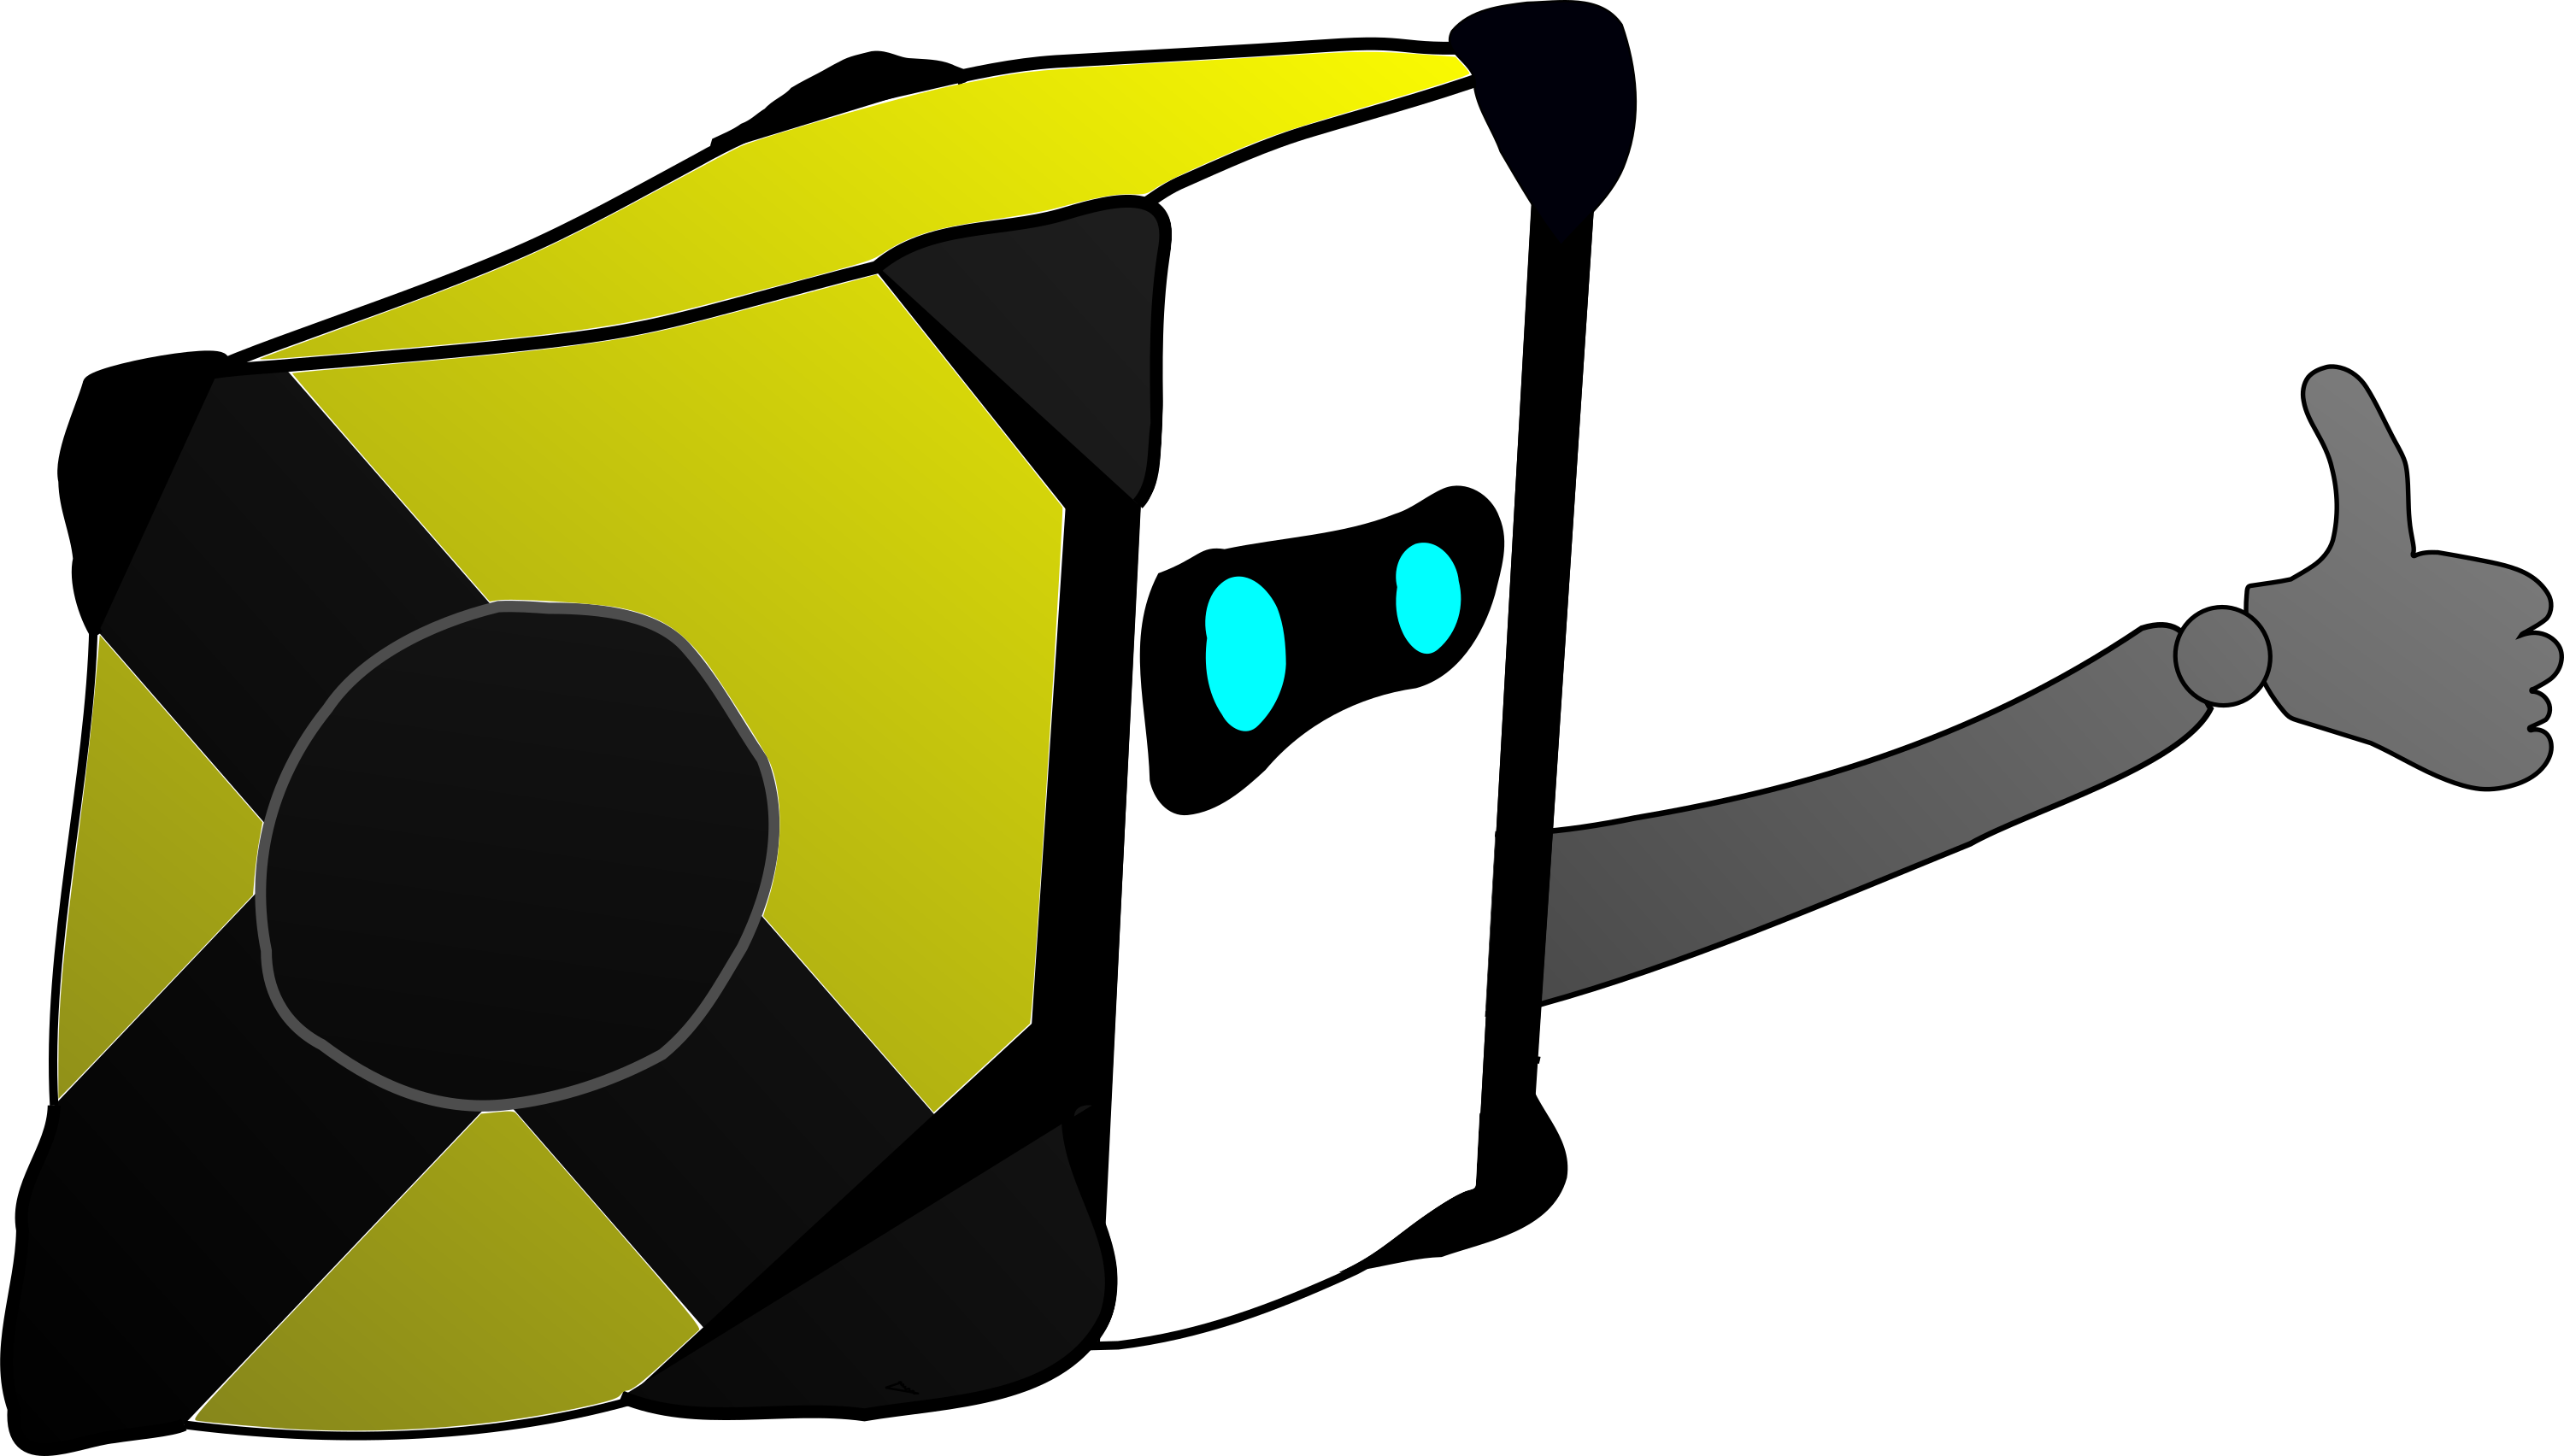
\includegraphics[width=8cm]{img/astrobee_mascot.png}
\end{figure}
\newpage

\tableofcontents

\newpage

\section{Introduction}

Astrobee is an autonomous micrgravity free-flyer, currently operating onboard the International Space Station (ISS) with the dual goal of helping astronauts with everyday activities while also serving as a microgravity autonomy research testbed. Astrobee uses an impeller-based propulsion system to direct air through multiple controllable vents in order to move around the interior of the ISS. Astrobee is also a capable modern robotics platform, operating with three processors networked together using the Robotic Operation System (ROS). Astrobee has three planned ISS units, an ISS docking port, and an accompanying ground facility with multiple prototype Astrobees and a ground station.

Fortunately, Astrobee's core flight software is entirely open source and includes a dedicated simulation environment, ready-to-go. That is where this guide comes in---to fill the gap between receiving access to these wonderful resources and getting new code integrated with Astrobee's flight software for simulation, ground, and eventual ISS experimentation. A high-level overview of these resources is provided in this section, and the remainder of this guide flows from initial setup to advanced ISS hardware preparation.

\subsection{Astrobee}
Astrobee is an autonomous free-flying robot designed to operate in microgravity, as shown in Figure \ref{fig:astro}. As stated in the introduction, Astrobee has ground and ISS facilities and a simulation environment designed to mimic both of these environments as closely as possible. The Astrobee units on the ISS are named honey, bumble, and queen, and also use these names in simulation to differentiate between units. The many papers mentioned in the front matter are excellent resources for more detailed specifics on Astrobee's hardware capabilities and design intent---some key details for GNC purposes are provided in Section 2.

\begin{figure}[h!]
    \centering
    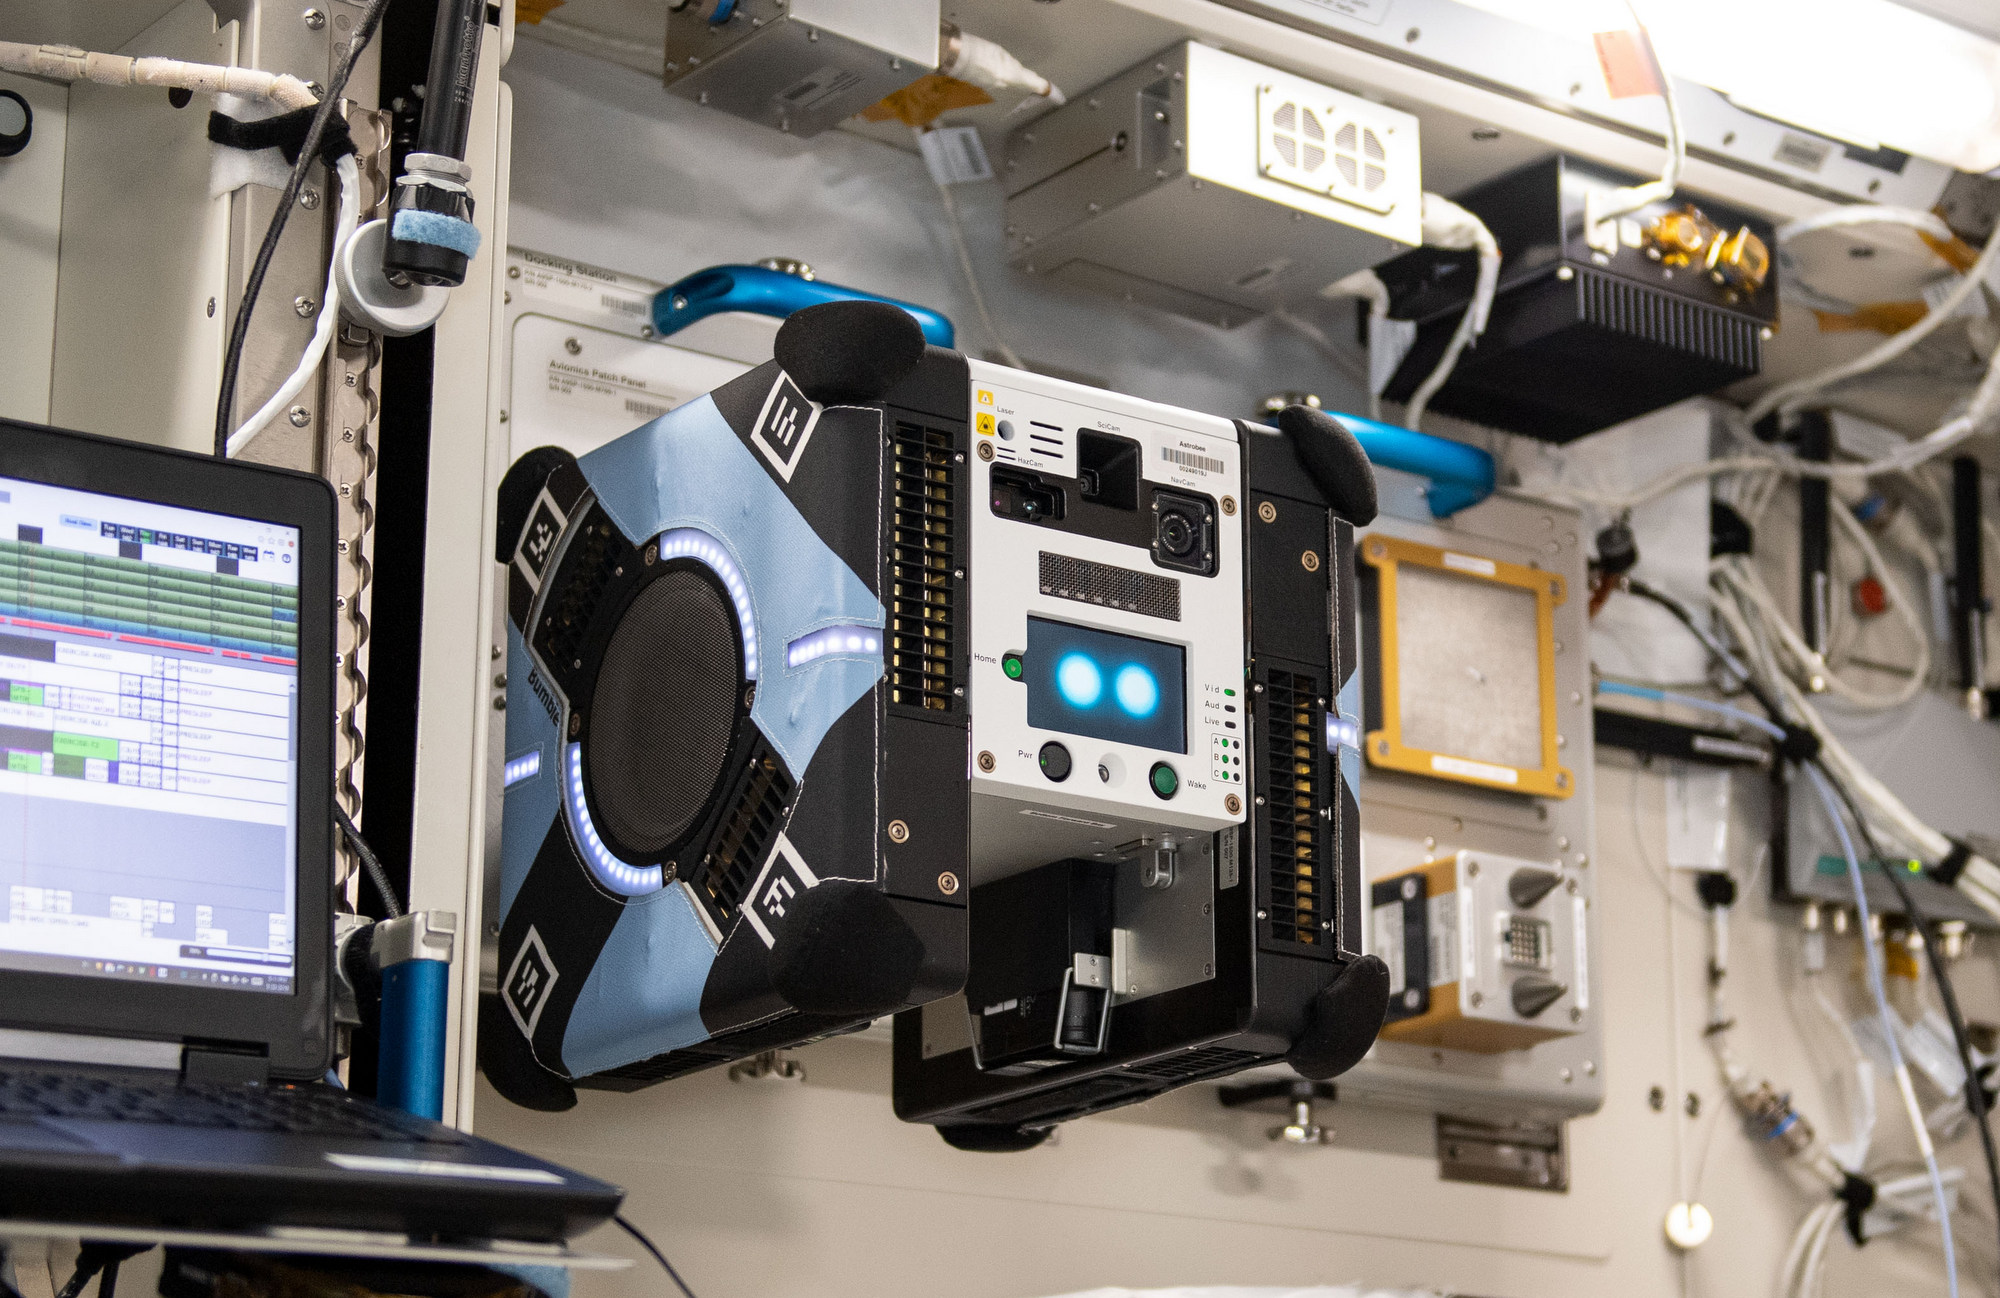
\includegraphics[width=0.8\textwidth]{img/nasa_astrobee.jpeg}
    \caption{The Astrobee free-flyer, at its docking port on the International Space Station. Three Astrobees are ultimately planned for use on-orbit. Image credit: NASA.}
    \label{fig:astro}
\end{figure}


\subsection{Astrobee Flight Software, Astrobee Android}

Each Astrobee has three processors onboard:
\begin{itemize}
    \item a high-level processor (HLP) running Android Nougat
    \item a mid-level processor (MLP) running Ubuntu 16.04 with ROS Kinetic
    \item a low-level processor (LLP) running Ubuntu 16.04 with ROS Kinetic
\end{itemize}

Specifics on the processors may be found in Fluckiger et al. \cite{Fluckiger}. The HLP differs from the MLP and LLP in that it is not Ubuntu-based and is meant to host Guest Science applications written as Android APKs. The software running on the HLP is called \textit{Astrobee Android} and its code is also available publicly \href{https://github.com/nasa/astrobee\_android}{here}.

Astrobee Android is fundamentally different from the Astrobee Flight Software and is mainly intended as a driver manager for some human-robot interaction hardware and as an interface for Guest Science APKs to the lower-level autonomy capability. There is a separate guide for this interface to Astrobee, which can be found in the Astrobee Guest Science Program guide \cite{NASAAmesResearchCenter2017a}.

Meanwhile the Astrobee Flight Software (AFS) is primarily coded in C++ and encapsulates key functionality in ROS nodelets. The AFS runs on the MLP and LLP, with the LLP primarily handling tasks that are closer to the hardware, e.g., control. AFS source code and some documentation in the form of README files can be found \href{https://github.com/nasa/astrobee}{here}. AFS contains the key autonomy functionality including motion planning, mapping, control, and high-level decision-making and is the focus of this guide; setup instructions are detailed in Section 3.

\subsection{Astrobee Simulation}
The Astrobee Flight Software comes with the Astrobee simulator. Single or multiple Astrobees can be simulated in an ISS or granite table environment. The robot's propulsion system, inertial and camera sensors, and  perching arm are simulated, along with all associated drivers. The simulator code is in the form of Gazebo plugins which recreate input seen on the actual Astrobee hardware. This allows testing of new code prior to its deployment to hardware, using the same ROS framework that is actually used on hardware. An example screenshot of the simulation is shown in Figure \ref{fig:sim}. Section 4 covers some key simulation concepts.

\begin{figure}
    \centering
    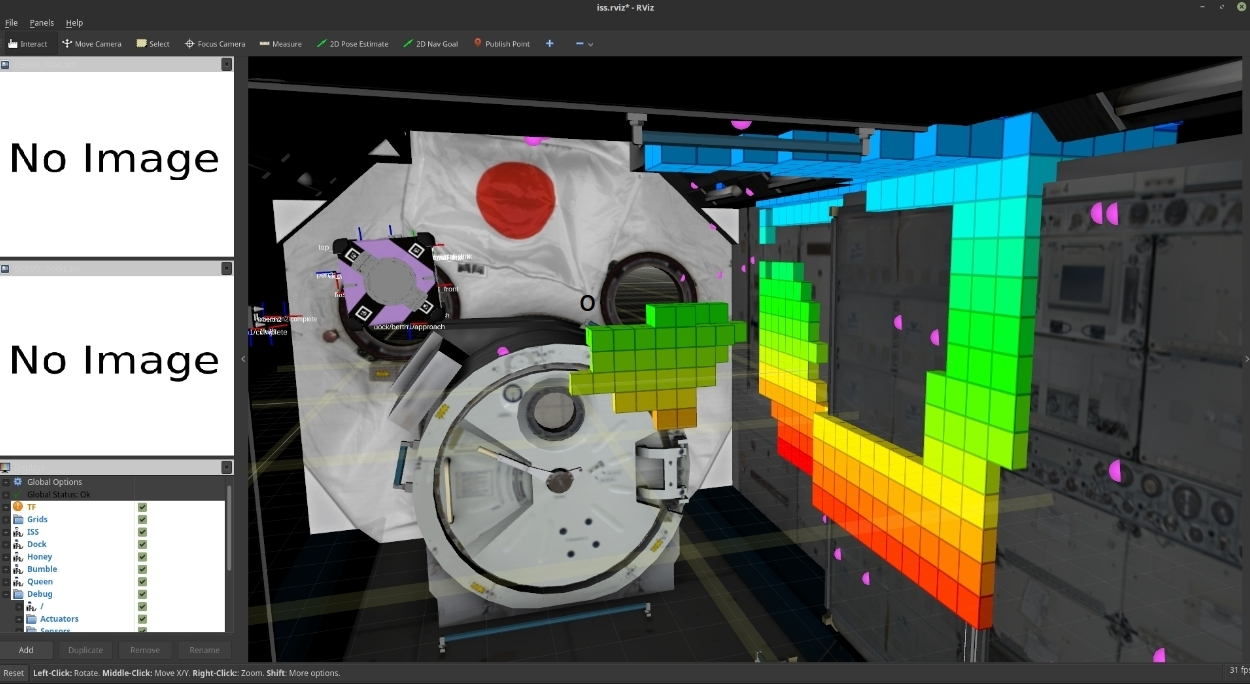
\includegraphics[width=\textwidth]{img/sim.jpg}
    \caption{An example of the Astrobee simulation in action, here showing a single Astrobee producing a voxel map based on depth camera measurements.}
    \label{fig:sim}
\end{figure}

\subsection{GDS}
The Ground Data System (GDS) is a graphical user interface and command software for Astrobee used from control stations on the ground or the ISS. Commands are sent over the  Data Distribution Service (DDS) protocol. DDS commands are converted to ROS commands onboard Astrobee by the AFS to be communicated to the robot by the DDS bridge. It also subscribes to ROS messages useful for monitoring the robot and sends them to ground as DDS messages. GDS is discussed briefly in Section 8 in the context of integration for ISS testing.

\clearpage
\section{Configuration}

Astrobee's physical parameters and environment must be known for control, estimation and planning. These parameters are approximately known for the actual hardware, and are also modifiable in the simulation environment. A set of configuration files can be found in \texttt{astrobee/config}.\footnote{Directories throughout the guide are referred to with respect to the Astrobee source code directory. A directory listing is shown in Appendix \ref{section:directory}.} These config files set many default robot parameters (including physical parameters), some of which are reset via launch files. There is not much documentation on these config files, but the inline coding is fairly self-explanatory. Note that \texttt{astrobee/config/worlds} contains some particularly useful config information. Finally, configuration information for Gazebo is also specified in URDF files, explained further below and in Section 4.

\subsection{Physical and Mass Properties}

In order to control the robot, it is necessary to know the system dynamics and parameters. Nominally, Astrobee obeys the rigid body dynamics of the Newton-Euler equations. Astrobee also has a small two degree of freedom robotic arm, whose use results in robotic free-flying dynamics. These dynamics are discussed in Chapter 3 of \cite{Albee2019} and are not shown here.

\subsubsection{Dynamics and State Vector}
For use not involving the arm, the Newton-Euler dynamics can be assumed:

\begin{align*}
\begin{split}
\mathbf{r} &= 
\begin{bmatrix}r_x&r_y&r_z\end{bmatrix}^\top\\
\mathbf{q} &=  
\begin{bmatrix}q_x&q_y&q_z&q_\theta\end{bmatrix}^\top\\
\mathbf{v} &=
\begin{bmatrix}v_x&v_y&v_z\end{bmatrix}^\top\\
\bm{\omega} &=
\begin{bmatrix}\omega_x&\omega_y&\omega_z\end{bmatrix}^\top\\
\end{split}
\quad \quad \mathbf{x} = 
\begin{bmatrix}\mathbf{r}\\\mathbf{q}\\\mathbf{v}\\\bm{\omega}
\end{bmatrix}
\end{align*}

\begin{align*}
&\mathbf{\dot{r}}_{CoM} = \mathbf{v}\\
&\mathbf{\dot{v}}_{CoM} = \frac{\mathbf{F}}{m}\\
&\mathbf{\dot{\bm{\omega}}} = -\mathbf{I}^{-1}\bm{\omega}\times\mathbf{I}\bm{\omega} + \mathbf{I}^{-1}\bm{\tau}\\
&^{I}_{B}\mathbf{\dot{q}} = \frac{1}{2} \bar{\mathbf{H}}(^{I}_{B}\mathbf{q})^{\top} {^{B}\bm{\omega}_{IB}}
\end{align*}

\noindent where $\mathbf{x}$ is the state vector, $\mathbf{r}$ is position, $\mathbf{q}$ is orientation (a quaternion, representing the body frame orientation with respect to the inertial frame), $\mathbf{v}$ is linear velocity and $\bm{\omega}$ is angular velocity (in the body frame). $\mathbf{F}$ is the 3-vector of applied force (for Astrobee this is defined in the \textit{body} frame!) and $\bm{\tau}$ is the 3-vector of applied torque. $\mathbf{I}$ is the inertia tensor, and $m$ is the mass. Finally, $\bar{\mathbf{H}}$ is a quaternion conversion matrix, defined explicitly in \cite{Albee2019}. It is assumed that the body frame is at the center of mass, $CoM$.

The state vector estimate, $\mathbf{\hat{x}}$ can be obtained on the topic \texttt{gnc/ekf}, under the EkfState message. Simulation ground truth of $\mathbf{x}$ can be obtained on the topics \texttt{loc/truth/pose} and \texttt{loc/truth/twist}. Consult Section 5 for further details.

\subsubsection{Inertial Parameters}

Gazebo ground truth parameters are set in their respective URDF files, specified in \texttt{description/description/urdf}. The mass esimates are ``fairly accurate," the moment of inertia estimates are ``somewhat accurate." Values for ground air bearings are only ``somewhat accurate." See Section 4 for more details on the URDF description files.
\\

The current mass estimate is $m = 9.58\ $kg.
\\

The current inertia tensor estimate is:
\begin{align*}
    \mathbf{I} =  
    \begin{bmatrix}
              0.153 & 0 & 0\\
              0 & 0.143 & 0\\
              0 & 0 & 0.162
    \end{bmatrix}  \text{kg-m}^2\\
\end{align*}

\noindent Note that in reality these values will differ for each Astrobee and have an inherent uncertainty. These parameters will likely be updated at some point in the future. These parameters are published to the ROS topic \texttt{mob/inertia}.

\subsection{Constraints}
\subsubsection{Position and Velocity Constraints}

Position constraints are not necessarily enforced by any default Astrobee planner (planner\_qp, however, does obey keep-in/keep-out zones, but not all of them.). \texttt{astrobee/resources/zones} has the latest ISS and granite table zones, written as serialized ROS messages. To obtain nominal position constraints these zones can be converted to message form and analyzed.

By default, Astrobee uses a $\pm 0.1 \ \frac{\text{m}}{\text{s}}$ velocity constraint.

\subsubsection{Force and Torque Constraints}

The quoted max thrusts per axis at various impeller fan speeds are given in Table 1. These maximum forces values are approximate and will likely be updated at some point in the future.

\begin{table}[h!]
\centering
\begin{tabular}{ |c|c|c|c| } 
    \hline
    Motor Speed [RPM]& x-axis [N]& y-axis [N]& z-axis [N] \\
    \hline
    2000 RPM & 0.452 & 0.216 & 0.257 \\
     \hline
    2500 RPM & 0.680 & 0.332 & 0.394 \\
     \hline
    2800 RPM & 0.849 & 0.406 & 0.486 \\
     \hline
\end{tabular}
     \label{table:speeds}
     \caption{The approximate thruster maximum forces per axis.}
\end{table}

\noindent Astrobee's thruster offset is about $0.1\ \text{m}$ from the $CoM$, so the torque limit is very roughly about $\frac{1}{10}$ of each of these values (each vent produces approximately half of the max force). These are only approximations for the torque limits, and will likely be updated at some point in the future.
     
\subsection{Mixing Matrix (Mixer)} 
Astrobee has a holonomic thruster placement, with 12 independent thrust vents. Vents on the X-axis have the largest nozzles and have the maximum acceleration capability, as Table 1 shows. A thruster placement diagram and explanation is given in \cite{Smith2016}. Most of the GNC pipeline, including the force allocation module (FAM) was originally implemented in Simulink for the Astrobee simulator. The physical properties of the impeller and the nozzles, such as the nozzles' minimum/maximum open angles, etc. can be found in this model, located at\\ \texttt{gnc/matlab/physical\_props/abp\_astrobee\_physical\_properties\_init.m}. However, a derivation of the mixing matrix (a mapping from desired inputs to vent angle) is not currently available and will likely be updated at some point in the future.



\subsection{Worlds and Coordinate Conventions}
By default Astrobee has two worlds (simulation environments), granite and ISS. Each world has an inertial coordinate frame, and ROS' standard tf2 package is used for tracking coordinate frames.
\\\\
\begin{markdown}
**Note: If the simulation environment has been changed, the accelerometer bias must be reset. This can be done by running**

~~~~
rosrun executive teleop_tool -reset_bias
~~~~
\end{markdown}


\subsubsection{Granite}
The granite world mimics the granite table in use at the NASA Ames ground test facility. The Ames table is $2 \times 2\ \text{m}$, though tighter constraints are in place at the actual test facility. The coordinate system mimics that of the ISS, where z+ is toward GND (down), shown in Figure \ref{fig:sim_axes}.

\subsubsection{ISS}
The ISS world is a mockup of the US Segment of the International Space Station. By default, Astrobee is docked in the Japanese Experiment Module (JEM) of this segment. The approximate volume of this segment is $1.5 \times 6.4 \times 1.7\ \text{m}$, in ISS coordinates. The coordinate system is shown in Figure \ref{fig:sim_axes_iss}.
\\\\
A good default location within the JEM for the ISS world is:
\begin{markdown}
~~~~
roslaunch astrobee spawn.launch dds:=false
robot:=sim_pub pose:="11.25 -6.95 4.49 0 0 0 1" 
~~~~~
\end{markdown}

\begin{figure}[h!]
    \centering
    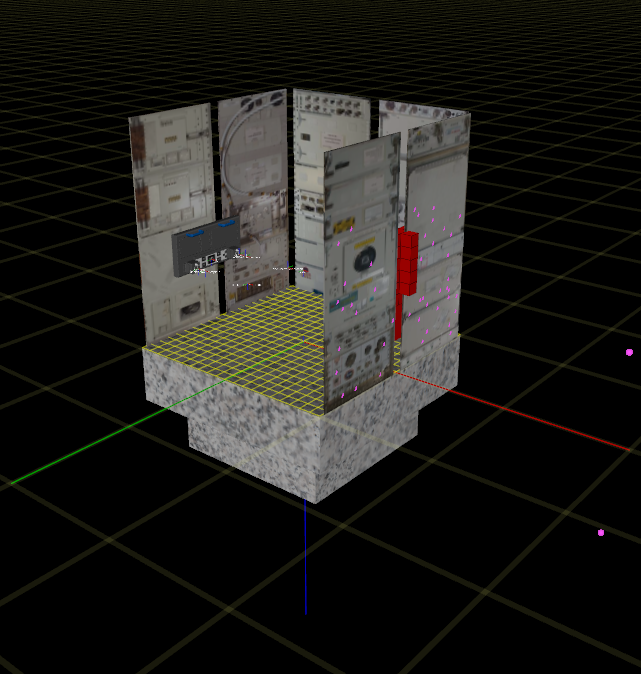
\includegraphics[height=10cm]{img/sim_axes.png}
    \caption{The coordinate convention for granite in use at the actual ground test facility. RGB corresponds to XYZ for the axes shown, where z+ points down.}
    \label{fig:sim_axes}
\end{figure}
\begin{figure}[h!]
    \centering
    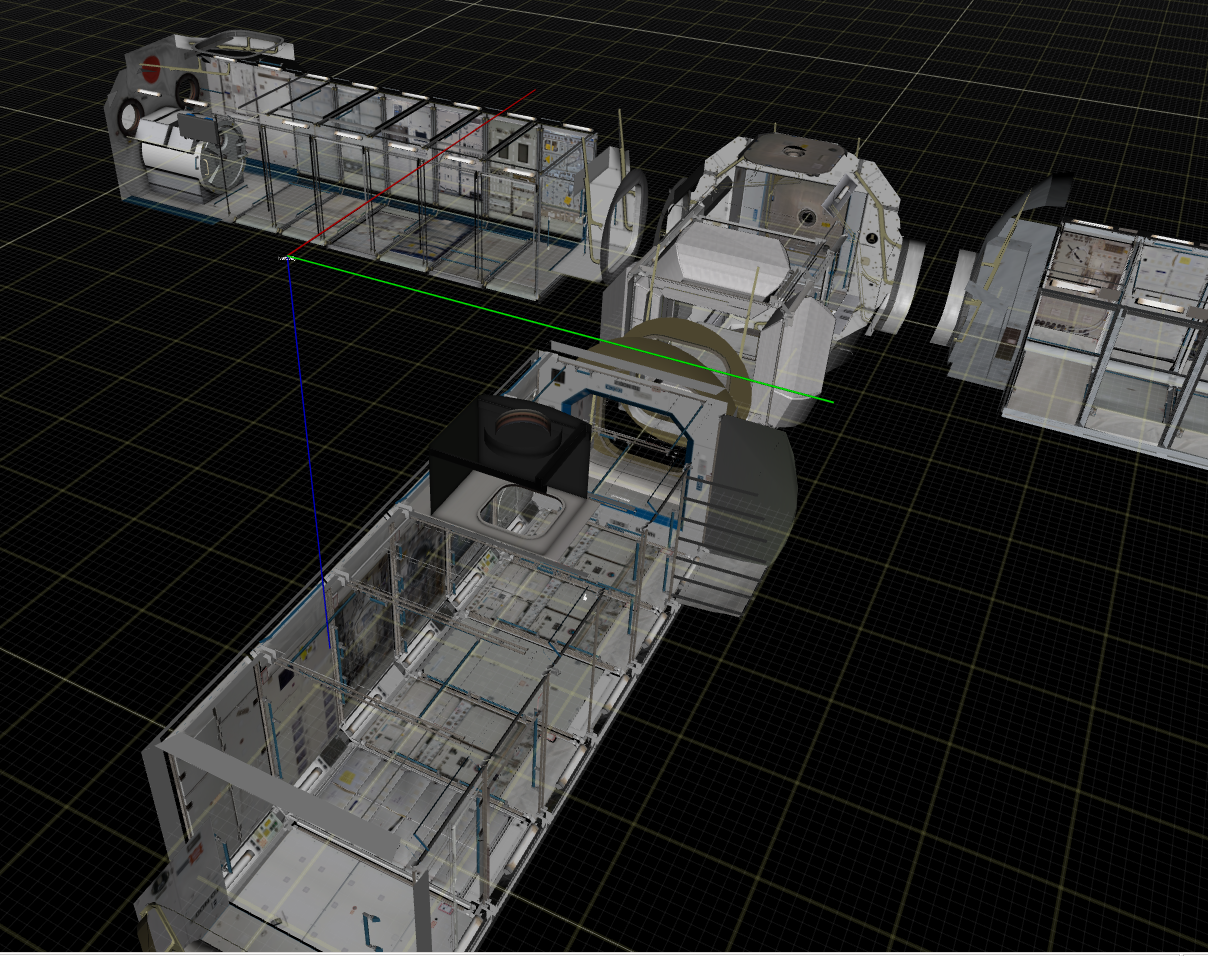
\includegraphics[height=10cm]{img/ISS_frame.png}
    \caption{The coordinate convention for ISS. RGB corresponds to XYZ for the axes shown. JEM is the module in the top left.}
    \label{fig:sim_axes_iss}
\end{figure}


\clearpage
\section{Setup, Building, and Running the Flight Software} 

Astrobee's public-facing, external flight software code is available \href{https://github.com/nasa/astrobee}{here}. This code is what is actually run on the robots, minus a few NASA internal directories. Some guides are available within that repository that will help with getting the simulation up and running---the instructions in \texttt{INSTALL.md} specifically will help with this. Many \texttt{README.md} files within the code also provide useful documentation. For completeness, install instructions are also provided here with some additional guidance to help with some common sticking points. The Astrobee simulation \textit{requires} Ubuntu 16.04 (but unofficially supports 18.04 and Linux Mint based on 16.04 and 18.04)---the instructions that follow assume the user has a clean Ubuntu 16.04 installation and is ready to use the terminal.

\subsection{Setup}
First, the source code directory, build directory, and install directory must be placed somewhere. The recommenced structure is shown in Figure \ref{fig:my_label}, where the source code cloned from NASA's repository is in \texttt{freeflyer-shared}.\footnote{As a reminder, most directories mentioned in this guide are relative to the main source code directory, \texttt{freeflyer-shared}.} Note that it is possible to name this directory as desired: \texttt{freeflyer-shared} is just a convention.

\begin{figure}[h!]
    \centering
    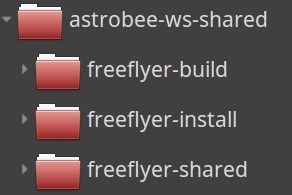
\includegraphics[height=130px]{img/astrobee_ws.jpg}
    \caption{The recommended folder setup for Astrobee. This is slightly different from the normal Catkin workspace structure the user might be used to when working with ROS.}
    \label{fig:my_label}
\end{figure}

\begin{markdown}
~~~~
git clone https://github.com/nasa/astrobee.git \$SOURCE_PATH
~~~~

e.g.,

~~~~
git clone https://github.com/nasa/astrobee.git freeflyer-shared
~~~~
\end{markdown}

\vspace{0.5cm}
Scripts are available to install required debians (packages)---some of these packages are available from the normal Ubuntu repositories, others are created by AFS scripts and built specifically for the user's computer, and some must come from the ROS repositories. Three scripts accomplish this:
\begin{markdown}
~~~~
./scripts/setup/add_ros_repository.sh
./scripts/setup/debians/build_install_debians.sh
./scripts/setup/debians/install_desktop_16_04_packages.sh
~~~~
\end{markdown}

It is a good idea to have ROS check for additional dependencies:
\begin{markdown}
~~~~
sudo rosdep init
rosdep update
~~~~
\end{markdown}

\noindent As a non-NASA user some of these packages (related to use of the Ground Data System (GDS)) are unavailable---this is okay, but the user will notice that some packages are not found when running the installation scripts.

AFS uses CMake for its build system. In order to prepare a makefile for the entire project, the build must be configured from AFS' CMakeLists.txt files. NASA provides a configuration script to help with this---the user just needs to run the configuration script with the desired build and install directories. (Reminder: these paths are relative to \texttt{freeflyer-shared}):
\begin{markdown}
~~~~
./scripts/configure.sh -l -F -D -p $INSTALL_PATH -b $BUILD_PATH
~~~~

e.g.,

~~~~
./scripts/configure.sh -l -F -D -p ../freeflyer-install/native
-b ../freeflyer-build/native
~~~~
\end{markdown}
\vspace{0.5cm}
The recommended \texttt{\$INSTALL\_PATH} is \texttt{../freeflyer-install/native}. The recommended \texttt{\$BUILD\_PATH} is \texttt{../freeflyer-build/native}. 

CMake has generated the makefile and other necessary bits in the build directory after running \texttt{configure.sh}.

\subsubsection{Advanced Details, Ubuntu 18.04 and 20.04 Setup}

\noindent\textbf{Note: Skip these details unless interested in installing new external libraries or attempting to satisfy dependencies on a different Linux operating system.}
\\\\
Astrobee has a variety of external dependencies that must be available on the processors (and the user's simulation computer) for the flight software stack to work. NASA's setup instructions install (most) of these dependencies as debians, the standard package format for Ubuntu-based Linux systems. This is accomplished through two scripts, \texttt{scripts/setup/debians/build\_install\_debians.sh} and \texttt{scripts/setup/install\_desktop\_16\_04\_packages.sh}. Briefly, creating a debian package works in the following way:
\begin{enumerate}
    \item A normal directory full of source code and CMakeLists.txt is produced.
    \item A \texttt{debian} subdirectory is inserted.
    \item \texttt{control} and \texttt{rules} files are created inside the \texttt{debian} subdirectory in order to define dependencies and compilation instructions, respectively.
    \item The \texttt{debuild} command is used on the package directory to create a debian package.
    \item The \texttt{dpkg -i} command is used to actually install the debian according to the \texttt{*.install} instructions in the package directory. 
\end{enumerate}

Astrobee's setup process creates some of these debians on-demand and fetches some pre-prepared debians for installation. Advanced instructions on tweaking Astrobee's debian installation process (e.g., for installing dependencies on another distro) are explained in \texttt{scripts/setup/debians/readme.md}. On Ubuntu 18.04, for example, different \texttt{controls} and \texttt{rules} files are used, and an older version of OpenCV (3.3.1, which is found in ROS Kinetic) must be installed. The main difficulty the user might encounter is updating dependency versions or telling CMakeLists.txt that a specific dependency is required if multiple exist on a system. An example of a custom setup and build process is available in Appendix \ref{app:charles}.

\subsection{Building}

After setting up the directory structure, getting the source code, and configuring, it's time to begin building (compiling and linking) the source code. This process is a little different depending on whether the user is working with the simulation or the actual robot (cross-compiling).

\subsubsection{For Simulation}
After setup, to perform a first build or incorporate new source code changes into the Astrobee build, run:
\begin{markdown}
~~~~
make -j2
~~~~
\end{markdown} 

\noindent{}in the build directory, \texttt{freeflyer-build/native} for example. Note that \texttt{-j2} specifies the number of cores to run on---e.g., if the user has 8 cores and runs \texttt{make -j8} the code will build much faster.

What is the the build process doing? A few things---first, it checks to make sure a set of required libraries are installed. Some ROS messages are generated, media files are
loaded, and OGRE (a graphics engine used for some RViz visuals) is configured. Finally, C++ targets are built according to what is specified in the (long) makefile in 
\texttt{freeflyer-build/native}. Specific details can be found by analyzing the \texttt{CMakeLists.txt} files which start in the main source directory. To additionally install targets (i.e., place targets in the directories specified by \texttt{CMakeLists.txt}), the user can run:

\begin{markdown}
~~~~
make install -j2
~~~~
\end{markdown}

Build targets are placed in \texttt{freeflyer-install}, though this is not necessary for just working in simulation.

\subsubsection{For Hardware}

The cross-compile build to be uploaded to Astrobee hardware requires a bit of extra work in order to cross-compile ARM-compatible targets. Detailed instructions are in \texttt{NASA\_INSTALL.md}.

Directories for the chroot (a directory mimicking the ARM file system) and toolchain (the actual tools used to cross-compile) must be specified. One option is to just put this working directory in the freeflyer workspace:

\begin{markdown}
~~~~
export ARMHF_CHROOT_DIR=$YOUR_CHOICE/arm_cross/rootfs
export ARMHF_TOOLCHAIN=$YOUR_CHOICE/arm_cross/toolchain/gcc
~~~~
\end{markdown}

\texttt{NASA\_INSTALL.md} details the further steps needed to do a cross-compile build for ARM. Those instructions are for NASA users only, however. An example native ARM build process is outlined in Appendix \ref{app:charles}.

\subsection{Running}
The Astrobee ROS workspace environment must be overlaid for ROS to find it. This can be done by sourcing the workspace setup file:
\begin{markdown}
~~~~
source $BUILD_PATH/native/devel/setup.bash
~~~~

\end{markdown}

As a first sample test of the simulation, the user can start up the standard sim using:

\begin{markdown}
~~~~
roslaunch astrobee sim.launch dds:=false robot:=sim_pub rviz:=true
~~~~
\end{markdown}

\noindent The simulation's RViz visualization should display in the ISS world.

It is possible to interact from the command line using \texttt{rosrun} or \texttt{roslaunch} to start up sets of nodes. Astrobee uses ROS for most of its message-passing, so interacting similarly as with a normal ROS environment is possible. It is also possible to use a script that will run the desired ROS commands so that command line updates aren't required, or to write a custom node(let) that interacts with the desired topics. Again, Astrobee runs on ROS: the hard part is finding exact details on which node(let)s do what, and what their interfaces are. For the autonomy pipeline, these details are covered in Section 5.

The user can also interact with Astrobee via NASA's ground data system (GDS) software. GDS is open-sourced \href{https://github.com/nasa/astrobee_gds}{here}, but its underlying DDS libraries are NASA-internal. GDS provides a GUI interface and convenient communications with Astrobee, and by default can support Guest Science interfacing with guest Android APKs or Java code---some additional details can be found in Section 8.



\subsection{Special Procedures for non-NASA Hardware Users}

If working on setup with the goal of eventually developing for custom hardware, then the user will need to follow some additional instructions. The MIT Space Systems Lab (SSL), for example, has a custom hardware setup using different processors and operating systems. Appendix \ref{app:charles} has an example of these special instructions for custom configuration on MIT's processors and may be useful for other custom hardware setups. 

\newpage
\section{Using the Simulation and Gazebo}

With AFS and the simulation environment set up from Section 3, it is now possible to begin working with the simulation, which is powered by Gazebo. Gazebo is the simulation backend (physics, visualization, etc.)---it is tightly integrated with ROS and does not require any setup beyond setup steps followed in Section 3. Note that NASA documentation for the simulation is growing and that \texttt{simulation/README.md} is another helpful resource.


\subsection{Launching the Sim}

A ROS launch file starts up a number of nodes (in Astrobee's case, nodelets) at the same time. The Astrobee simulation starts from a cascade of these launch files. The \texttt{astrobee/launch/sim.launch} file is the default starting point to run the simulation:

\begin{markdown}
~~~~
roslaunch astrobee sim.launch dds:=false robot:=sim_pub rviz:=true
~~~~
\end{markdown}

Default robot and DDS arguments are required for non-NASA usage. Flags and more information can be found \href{https://github.com/nasa/astrobee/blob/master/simulation/sim\_overview.md}{here}.


\subsection{Launch Sequence}

Astrobee is launched using a series of cascading launch files, as above. The sequence of these launch files is given in Figure \ref{fig:launchfiles}. \texttt{descriptions.launch} creates the environment and corresponding coordinate transforms; \texttt{spawn.launch} starts artificial drivers and nodes running on the LLP and MLP; \texttt{sim\_start.launch} begins the Gazebo and RViz simulation environments. 

\begin{figure}[h!]
    \begin{adjustwidth}{-1in}{-1in}
    \centering
    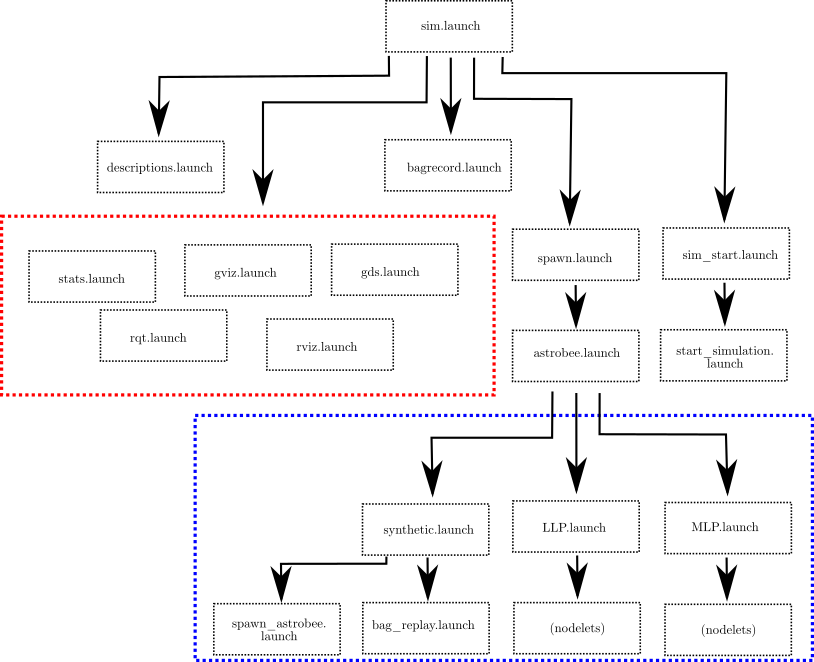
\includegraphics[width=1.4\textwidth]{img/launch_diag.png}
    \caption{The nominal Astrobee launch file sequence. The entry point to starting the simulation is \texttt{sim.launch}. A related launch file sequence is used to start up nodes on the actual hardware. Red indicates visualization launch files while blue indicates low-level driver and nodelet launch files.}
    \label{fig:launchfiles}
    \end{adjustwidth}
\end{figure}

Consult individual launch files for more details. Most launch files are found in \texttt{astrobee/launch}, but some are also located in \texttt{simulation/launch}. Individual packages also usually have their own launch files. Note that Astrobee uses special nodelets instead of nodes, which are able to pass messages more efficiently. Documentation on nodelets can be found \href{http://wiki.ros.org/nodelet}{here}, and additional details are provided in Section 7.


\subsection{Creating Objects, URDFs}

The \texttt{spawn\_astrobee} node located in \texttt{spawn\_astrobee.launch} \\
(located in \texttt{simulation/launch}) is used to bring Astrobee online in simulation. Parameter information is specified via xacro files, which are kept in \texttt{description/description/urdf}. These xacros are converted to URDFs by a parameter command in \texttt{astrobee.launch}. The \texttt{robot\_description} parameter contains the output of this command and is passed to the \texttt{spawn\_model} script in \texttt{simulation/scripts/spawn\_model}. The launch sequence is summarized in Figure \ref{fig:spawn}. The \texttt{model\_carriage*} xacros are only used if specified by launch file input arguments. Additional documentation on URDF and xacro files can be found \href{http://wiki.ros.org/urdf/XML}{here}.

\begin{figure}[h!]
    \begin{adjustwidth}{-0.5in}{-1in}
    \centering
    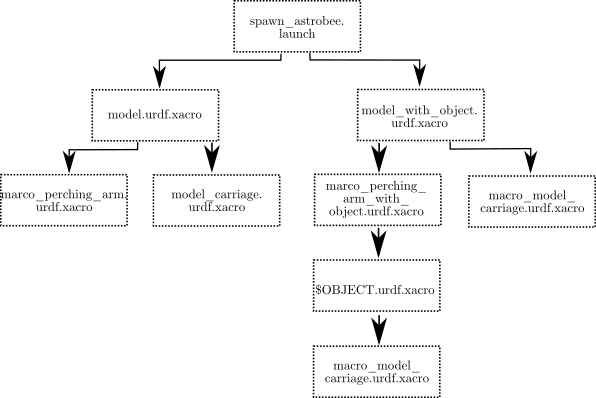
\includegraphics[width=1.3\textwidth]{img/urdf_diag.png}
    \caption{The Astrobee object spawning sequence. A sample ``with\_object" launch sequence that is not in the default simulation is also provided in this diagram. This spawn sequence is used to create objects in the sim, and can be modified as desired to include free-floating or rigidly attached objects.}
    \label{fig:spawn}
    \end{adjustwidth}
\end{figure}

\subsubsection{Attaching Rigid Objects}

Objects that are \textit{rigidly attached} to another model must have a URDF that is incorporated into the base. \texttt{model.urdf.xacro} contains an example of this process, including \texttt{macro\_perching\_arm.urdf.xacro} in its definition. Attaching a rigid object to another URDF (such as \texttt{model.urdf.xacro}) can be accomplished by mimicking this process.

\subsubsection{Free-floating Objects}

Free-floating objects can be spawned using a custom xacro and do not require interfacing with \texttt{model.urdf.xacro}. Just ensure that the Gazebo spawn is called from the launch file sequence.

\subsubsection{Multiple Objects}

Multiple URDF files with the same link name are a problem. This can be fixed by creating an xacro macro that wraps the xacro file, allowing for different parents, etc. to be specified. This would be required, for example, if \texttt{model\_carriage.xacro}, was used twice to describe an Astrobee and another object supported by a carriage.

\subsubsection{Global Static Objects}

The simulation uses a convention of ``global" transforms for objects that are static relative to the inertial ISS frame (e.g., the dock). Most of these objects are defined in \texttt{description/media/} and the ensuing subfolders. The actual transformations for these objects get set by the \texttt{framestore} node, which checks the config files (namely \texttt{iss.config} and \texttt{granite.config}) in order to set the necessary transformations relative to the ISS.

New global objects may be added to \texttt{framestore} for broadcasting, if desired.

\subsection{Visualization}

The Astrobee sim has RViz, SViz (Gazebo), GViz (GNC), and GDS visualizations. The RViz visualization is the most practically useful. Each of these can be started using the launch file input arguments specified \href{https://github.com/nasa/astrobee/tree/master/simulation}{here}.


\subsection{Multiple Astrobees}

Launching multiple Astrobees is possible using namespacing of topics. The Astrobee simulator can account for the following namespaces, currently: \texttt{/}, \texttt{honey}, \texttt{bumble}, and \texttt{queen}. `\texttt{/}' is the root namespace, and is the default when launching.
\\\\
Many default Astrobee command-line tools also accept the \texttt{-ns} argument, e.g.,

\begin{markdown}
`rosrun executive teleop -ns bumble -move -pos "4 0"`
\end{markdown}
\\\\
The \texttt{spawn.launch} launch file conjures up Astrobee in Gazebo and starts up namespaced nodelets. A namespaced Astrobee can be started using e.g.;

\begin{markdown}
`roslaunch astrobee spawn.launch ns:=honey pose:="1 2 3 0 0 0 1"`
\end{markdown}
\\\\
Additionally, \texttt{spawn.launch} namespacing options are available in the \texttt{sim.launch} file for calling up each platform, using arguments \texttt{honey}, \texttt{bumble}, and \texttt{queen}.

As an example, if running multiple Astrobees their respective topics must be properly namespaced so that they do not clash when run on a single machine. This can be accomplished using the \texttt{ns} argument when launching an Astrobee from a launch file. For example, the following will launch a set of Astrobee nodelets under the \texttt{honey/} namespace:

\begin{markdown}
~~~~
<group if="$(arg honey)">
<include file="$(find astrobee)/launch/spawn.launch">
  <arg name="robot" value="$(arg robot)" />      <!-- Type of robot      -->
  <arg name="world" value="$(arg world)" />      <!-- Execution context  -->
  <arg name="ns" value="honey" />                <!-- Robot namespace    -->
  <arg name="output" value="$(arg output)" />    <!-- Output for logging -->
  <arg name="pose" value="$(arg pose_honey)" />  <!-- Initial robot pose -->
  <arg name="spurn" value="$(arg spurn)" />      <!-- Prevent node       -->
  <arg name="nodes" value="$(arg nodes)" />      <!-- Launch node group  -->
  <arg name="extra" value="$(arg extra)" />      <!-- Inject extra nodes -->
  <arg name="debug" value="$(arg debug)" />      <!-- Debug a node set   -->
  <arg name="sim" value="$(arg sim)" />          <!-- SIM IP address     -->
  <arg name="llp" value="$(arg llp)" />          <!-- LLP IP address     -->
  <arg name="mlp" value="$(arg mlp)" />          <!-- MLP IP address     -->
  <arg name="dds" value="$(arg dds)" />          <!-- Enable DDS         -->
</include>
</group>
~~~~
\end{markdown}

However, on actual hardware each Astrobee is namespaced relative to the \texttt{/} namespace on their individual processors. This means that launch file namespacing is \textit{not} necessary on the actual hardware!


\subsection{Teleop}

A few mobility command-line commands can be issued using the Astrobee mobility's \texttt{teleop} tool to directly control Astrobee. See the \texttt{teleop} documentation in \texttt{mobility/README.md}. These are convenience commands that sequence together other Astrobee tools to provide functionality for the user e.g., moving point to point by calling the planner and underlying control, for example:

\begin{markdown}
~~~~
rosrun mobility teleop -move -pos "0.1 0.2"
~~~~
\end{markdown}



\clearpage
\section{The Autonomy Pipeline}

The Astrobee GNC is divided into a few main packages: CTL (control), EKF (estimation), and FAM (force allocation module/mixer), along with autonomy packages for localization and planning. EKF fuses localization and measurement information to produce a state estimate, which is used by CTL in correcting error. Desired waypoints for planning come from a designated planner, which is in turn managed by the \texttt{choreographer}. Finally, actual control inputs are produced using the FAM module which interfaces with the low-level hardware drivers. Meanwhile, a variety of other Astrobee nodelets run alongside this system to e.g., manage external communications. Locating the source files and identifying their ROS inputs and outputs is key to making low-level modifications to Astrobee's autonomy software. 

By default, Astrobee launches a set of control and estimation nodelets on the LLP. (See \texttt{astrobee/launch/robot/LLP.launch}.) Some higher-level nodes are launched on the MLP. (See \texttt{astrobee/launch/robot/MLP.launch}.) Figure \ref{fig:gnc} provides a high-level overview of this pipeline, along with a sample of overriding it using integrated code. 

\begin{figure}[h!]
	\centering
	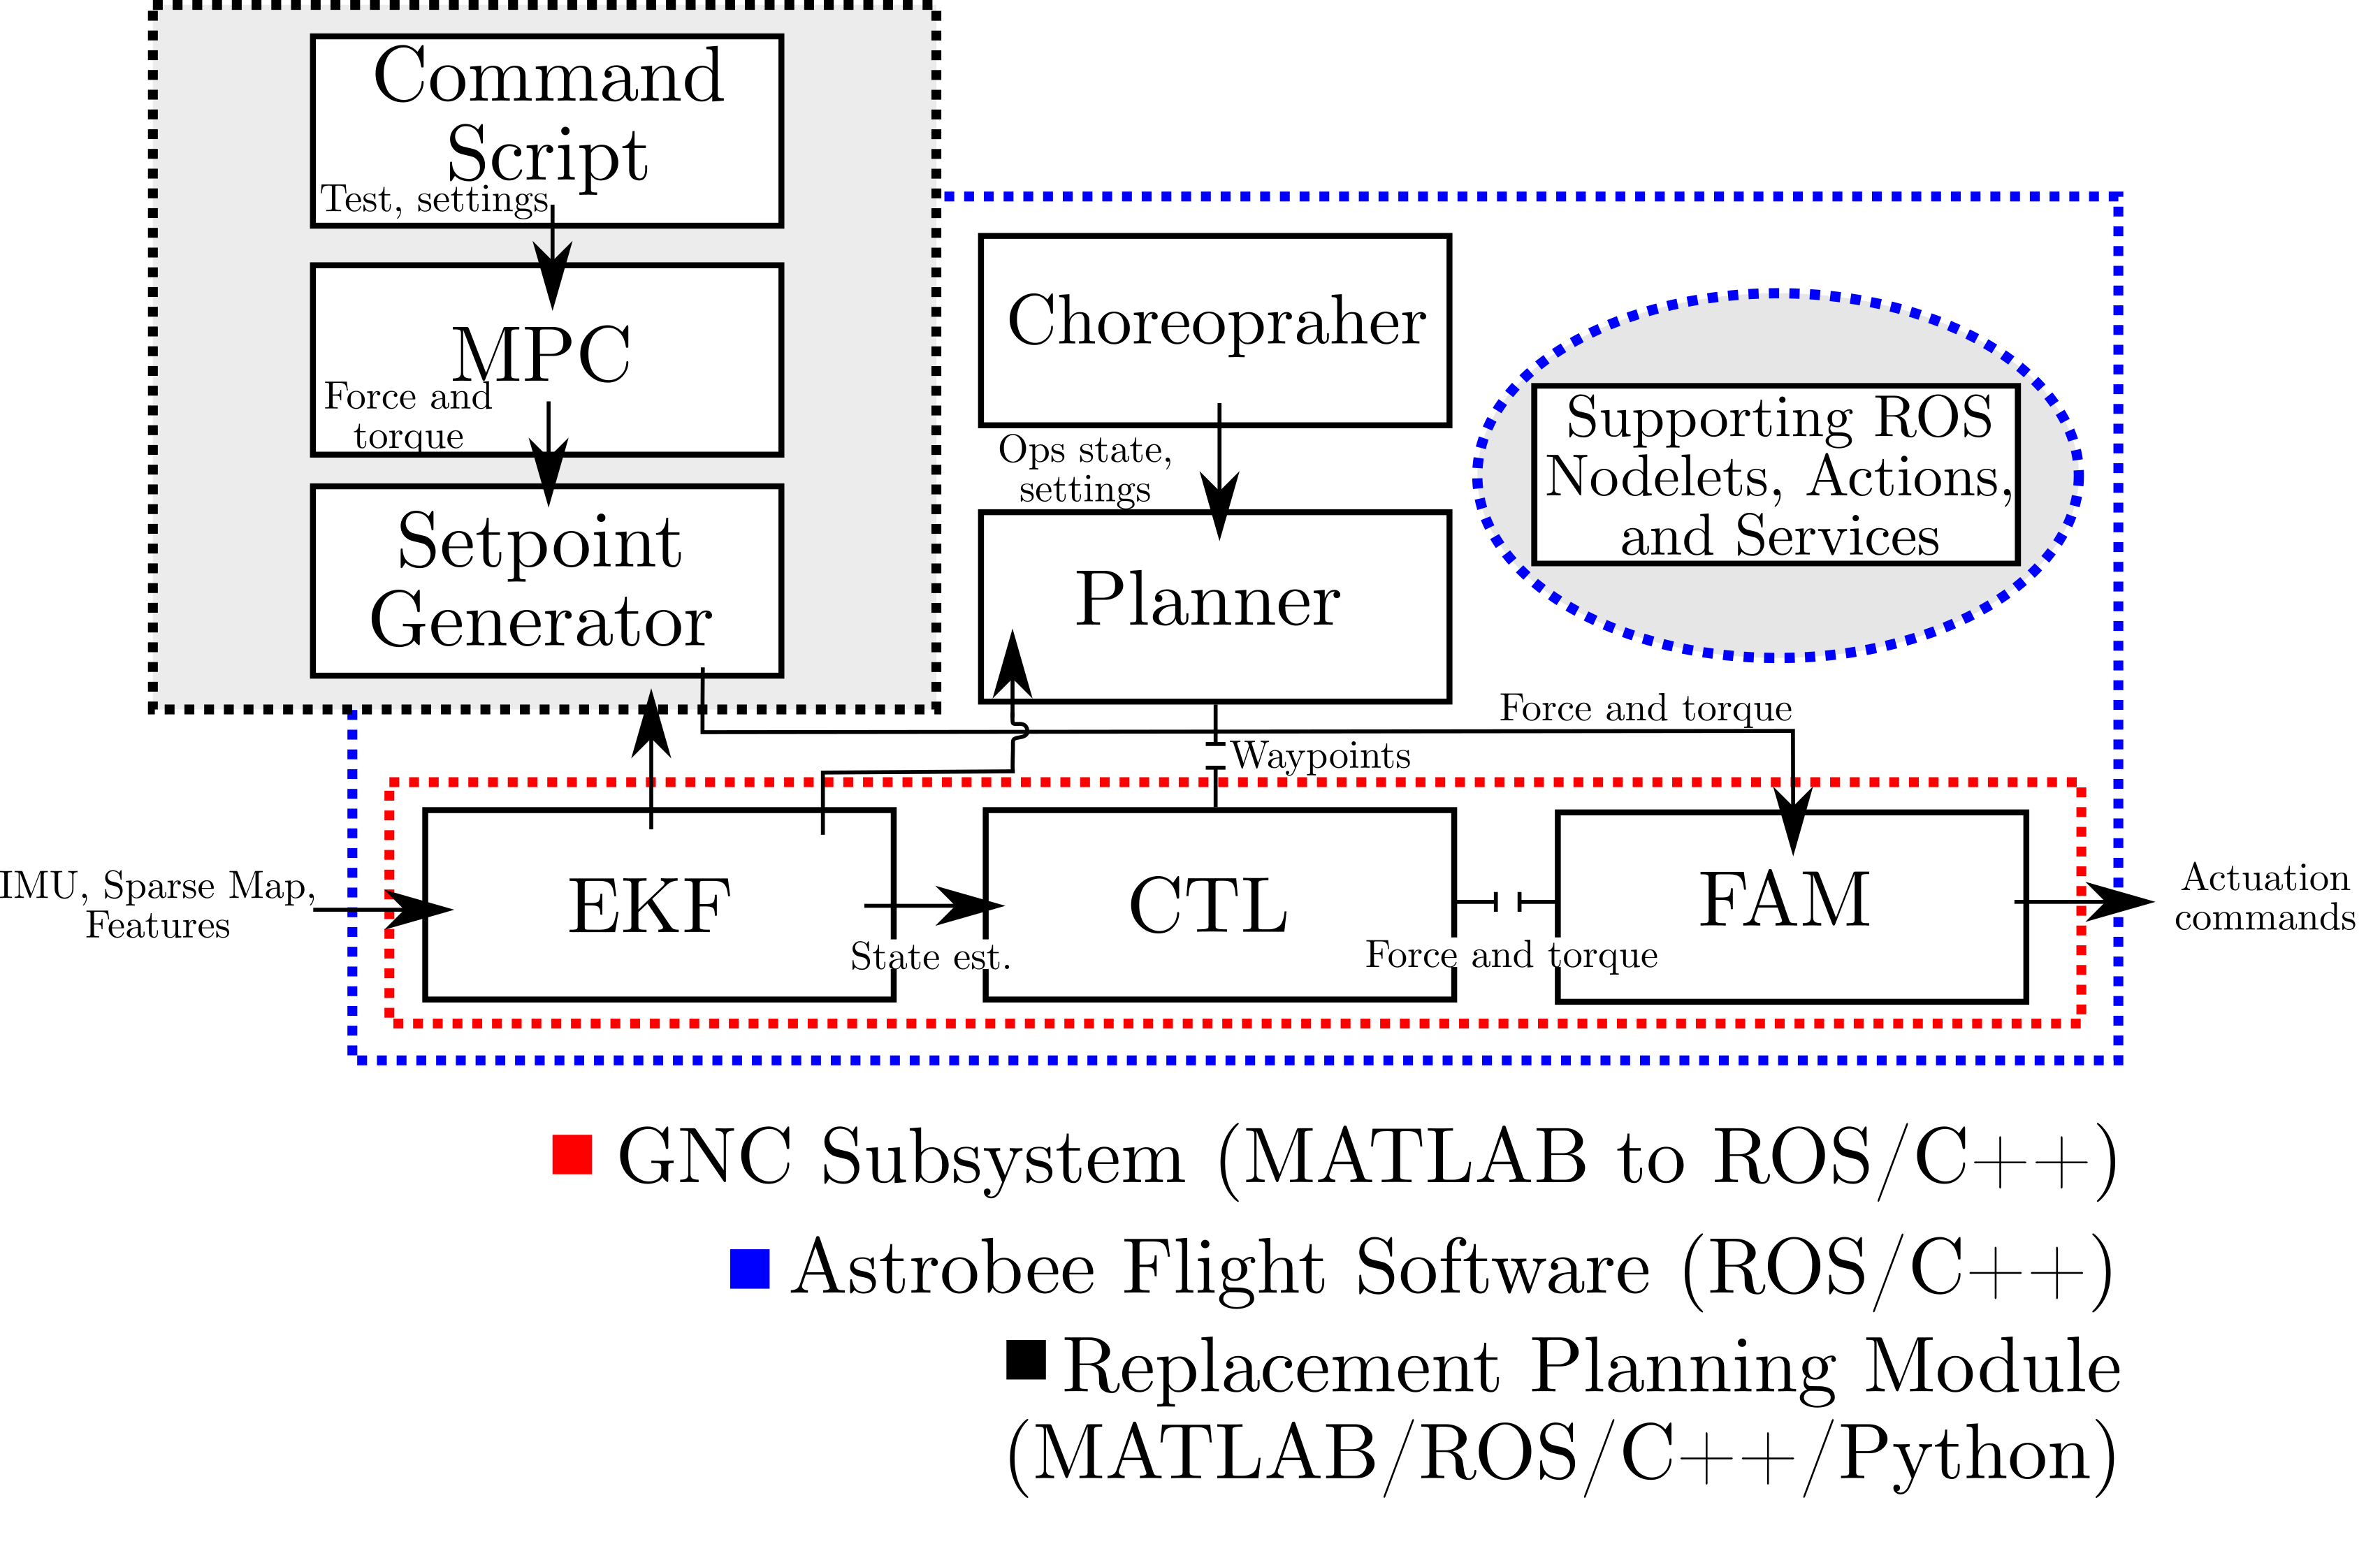
\includegraphics[width=1.0\textwidth]{img/Astrobee_GNC.png}
	\caption{An overview of the Astrobee GNC subsystem. The components outlined in black are an example of a \textit{replacement} pipeline overriding Astrobee's default GNC subsystem, which is outlined in red. This sort of customization is described further in this section.}
	\label{fig:gnc}
\end{figure}

\subsection{Locations of Key Parts of the Autonomy Pipeline}

Most of the CTL, EKF, and FAM code was autocoded from a MATLAB Simulink model (and is therefore somewhat hard to read as source code). This Simulink model can be found in \texttt{gnc/matlab/astrobee\_control\_sim.slx}. Also note that most packages have individual READMEs with additional information. For ease of reference, source code for portions of the pipeline can be found as noted here:

\begin{itemize}
 	\item High-Level Finite State Machine (FSM): \texttt{management/executive}
	\item Mobility FSM: \texttt{mobility/choreographer}
    \item Trajectory Planning: \texttt{mobility/planner\_*}
    \item Control: \texttt{gnc/ctl}
    \item Mixer: \texttt{gnc/fam}
    \item Estimation:  \texttt{gnc/ekf}
    \item Localization: \texttt{localization}
\end{itemize}


\subsection{Finite State Machines (FSMs)}

The \texttt{executive} and \texttt{choreographer} provide system-level and GNC-level management, respectively, often using their own FSMs to determine how to react. The exact logic behind decision-making is not covered here (it is intricate), but generally \texttt{executive} is useful from an autonomy perspective for getting external commands routed properly, and \texttt{choreographer} is useful for coordinating and monitoring interaction between GNC components (and interfacing with \texttt{executive}). Important information like inertial parameters and \texttt{flight\_mode} is also published by the \texttt{choreographer}. The general flow of information between these components is shown in Figure \ref{fig:FSMs}.

\begin{figure}[h!]
	\centering
	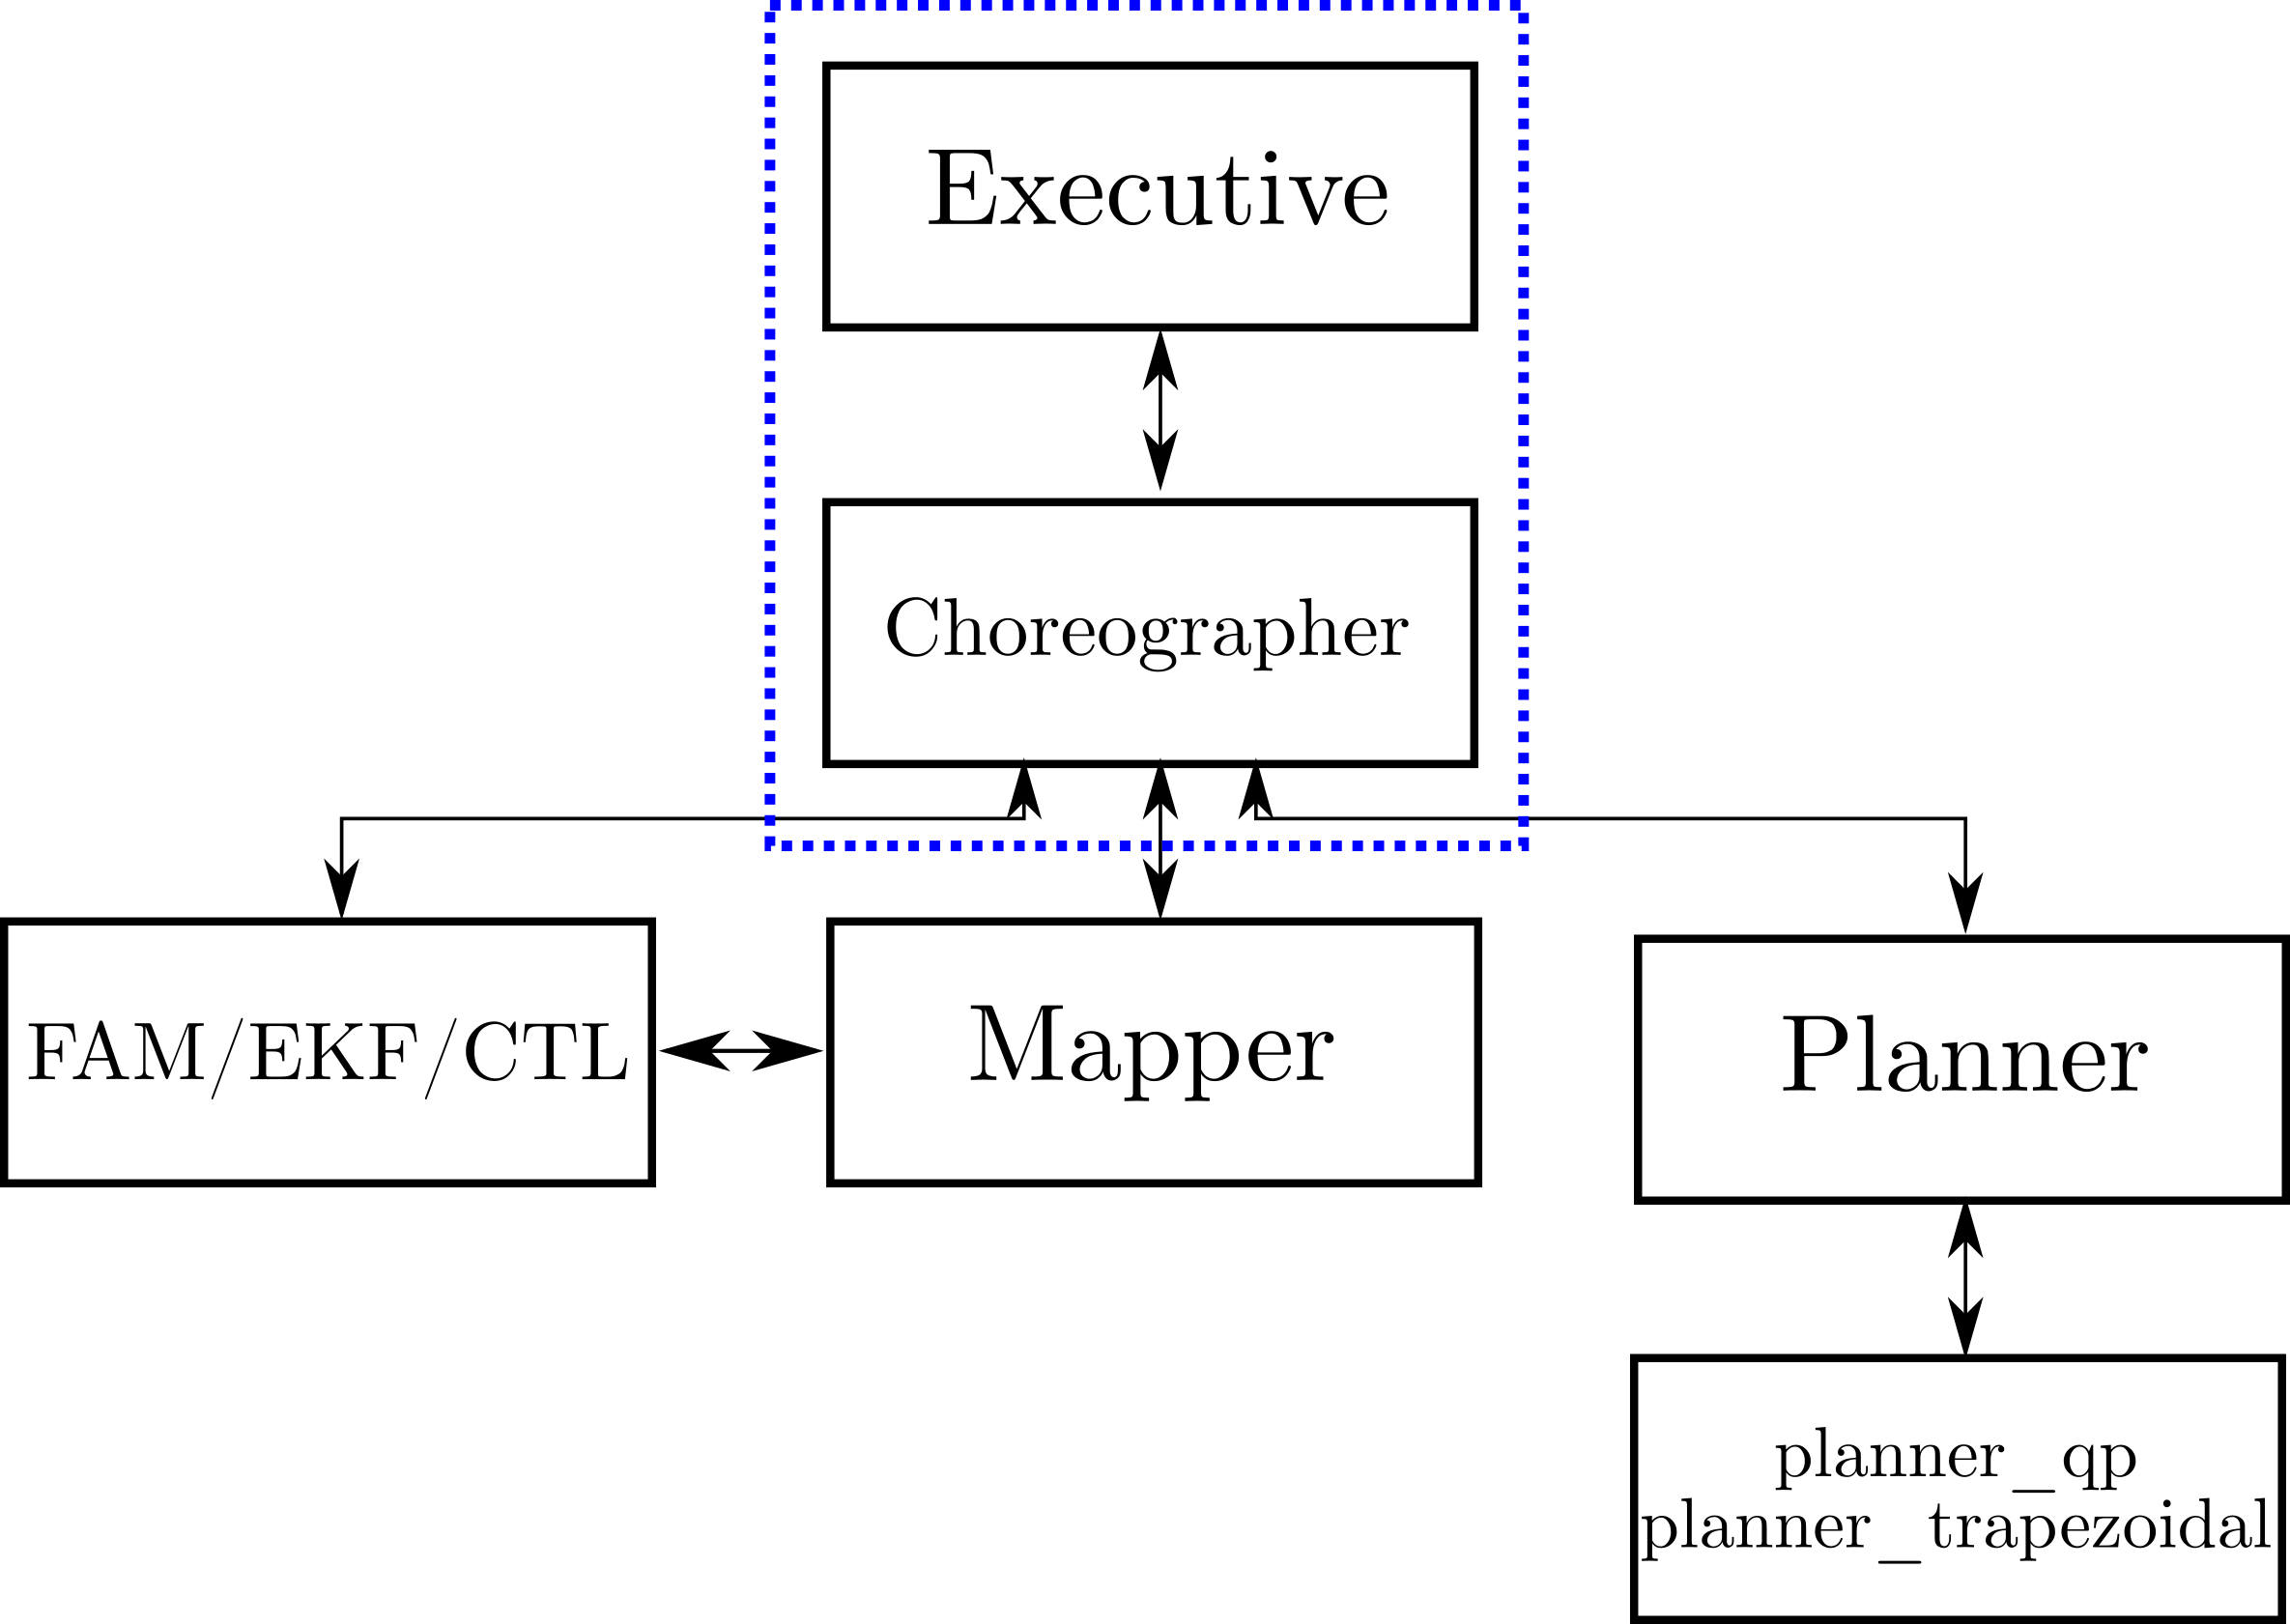
\includegraphics[width=1.0\textwidth]{img/fsm.png}
	\caption{A general overview of the interfacing between GNC components and the FSMs. The FSM-based nodelets are outlined in blue. (Based on NASA Ames AFS documentation.)}
	\label{fig:FSMs}
\end{figure}

\subsection{Planning}
\label{sec:plan}
Astrobee's default trajectory generators (planners) are directly coded in C++: there is no MATLAB autocoding. The goal of the planners is, given a goal state, to produce a set of dynamically-feasible trajectory setpoints. On top of that, the planners may optimize a cost function, or avoid obstacles. Only \texttt{planner\_qp} does both of these. The default planner, \texttt{planner\_trapezoidal}, creates straight-line trapezoidal velocity ramps and does simple obstacle checking---if an obstacle is in the way, it aborts. \texttt{planner\_qp} is a bit more sophisticated, and produces minimum-jerk, smooth, obstacle-avoiding trajectories \cite{Watterson2016}. There are two main ways to incorporate a new planner: (1) using the planner framework that the default planners uses or (2) bypassing the planning framework.

\subsubsection{Integrate into the Planner Framework}

This method requires the following:
\begin{itemize}
	\item Creating a new planner that inherits \texttt{planner::PlannerImplementation} (see \texttt{planner\_trapezoidal\_nodelet.cc} for an example)
	\item Filling in a minimal set of callbacks for a \texttt{planner::PlannerImplementation}
	\item Making sure \texttt{planner.h} is included, to register with \texttt{choreographer}
\end{itemize}

A finite state machine running in the mobility subsystem (\texttt{choreographer}) determines when and how planners are called, with configuration parameters also exposed via the \texttt{rqt\_reconfigure} ROS tool. Registration of a planner with \texttt{choreographer} makes a planner accessible to the \texttt{mob/motion} action. \texttt{mob/motion} is \textit{the} interface for calling a planner. It is used by the \texttt{teleop} tool and by other internal commands involving motion requests. \texttt{mob/motion} is aliased as \texttt{ACTION\_MOBILITY\_MOTION} in the codebase with action \texttt{ff\_msgs::MotionAction}. This action is made available by the \texttt{choreographer} nodelet upon launch. A detailed diagram of this process can be found in \texttt{doc/images/mobility}.

The flow of generating a trajectory and sending it out for control is:
\begin{itemize}
	\item \texttt{teleop} or \texttt{executive} calls \texttt{choreographer.Plan()} to initiate creating a trajectory (line 900 of \texttt{choreographer\_nodelet.cc}) via the \texttt{MotionAction}
	\item a request is sent to \texttt{planner.SendGoal()} (line 960 of \texttt{choreographer\_nodelet.cc})
	\item the planner action server calls its \texttt{GoalCallback()} (line 252 of \texttt{planner.h}) and calls the \texttt{PlanCallback()} (line 267 of \texttt{planner.h})
	\item the \texttt{PlanCallback()} routes the request to the trajectory generator defined by the planner implementation, and a \texttt{plan\_result} is set (e.g., line 85 of \texttt{planner\_trapezoidal\_nodelet.cc})
	\item separately, a request for control is made in \texttt{choreographer.Control()} (line 1068 of \texttt{choreographer\_nodelet.cc}) which publishes a goal to the control client. This call is made by the FSM, but the exact mechanism for specifying the rate of reading the plan is not clear
	\item CTL picks up the current action goal setpoint (line 343 of \texttt{ctl.cc}) and the segment is copied over to be processed
	\item a wrapper around the autocoded GNC uses the setpoint and current state to compute the required forces and torques, and sends them to the FAM (line 438 of \texttt{ctl.cc}), see \texttt{ctl.h} for the wrapper class definition. Note that \texttt{Control()} (line 400 of \texttt{ctl.cc}) actually sets the desired control state
\end{itemize}

\subsubsection{Bypass the Planner Framework}

It is also possible to bypass this framework entirely, if this acceptable for the intended use. If the user has their own trajectory generation scheme (in Astrobee parlance, a planner) you can avoid the FSM management from \texttt{choreographer} by simply publishing trajectory setpoints to the topic that \texttt{choreographer} would have ultimately published to. 

The following publishers can be made with roscpp: one for base controller setpoints, and another for the arm controller. This will route trajectory setpoints directly to the controller monitoring \texttt{TOPIC\_GNC\_CTL\_SETPOINT}.
 
\begin{markdown}
~~~~
//  Publish setpoints to base controller
pub_ctl_ = nh->advertise<ff_msgs::ControlState>(
TOPIC_GNC_CTL_SETPOINT, 5, true);

//  Publish setpoints to arm
pub_arm_ = nh->advertise<sensor_msgs::JointState>(
TOPIC_BEHAVIORS_ARM_SETPOINT, 5, true);
~~~~

`/gnc/ctl/setpoint` is aliased as `TOPIC_GNC_CTL_SETPOINT` in the codebase with message `ff_msgs::ControlState`.
\end{markdown}
\\\\
\indent Anecdotally, sending commands too frequently can make \texttt{ctl\_node} zero out commanded force. There is also a position tolerance violation if tracking is particularly poor. Its value can be changed in the config files. This can lead to entering a different mode, `stopping' mode. Finally, the user will need a way to run their setpoint publisher---in simulation, simply call via the command line or from another piece of code; for ISS use, one possibility is creating a custom command sent from GDS. Section 8 addresses some of these options.



\subsection{Control (CTL)}

The \texttt{ctl\_node} handles determining force/torques to send to the force allocation module (FAM), given the state of the system and a desired nominal trajectory. Within the original Simulink model, the closed loop control occurs at \texttt{astrobee/fsw\_lib/ctl\_controller/clc\_closed\_loop\_controller\_lib}.
The following topics are used:

\subsubsection{Inputs}
\begin{markdown}
* `gnc/ekf`: EKF state estimate.
* `gnc/ctl/control` An action specifying desired states for control.
\end{markdown}

\subsubsection{Outputs}
\begin{markdown}
* `gnc/ctl/command`: The force and torque commanded by control.
* `gnc/ctl/shaper`: The output from the GNC command shaper (smooths the control).
* `gnc/ctl/traj`: The desired trajectory.
* `gnc/ctl/segment`: The current segment of the trajectory.
* `gnc/ctl/progress`: The progress along the current segment.
\end{markdown}

\subsubsection{Bypassing the Controller Framework}

If the user wants a more general integration method that does not use the default Astrobee control framework (actions, state machines, etc) it is possible to publish directly to the mixer (FAM) (and arm, if desired). Otherwise, the default control scheme can then be tweaked to use incoming setpoints as desired. However, the default controller is a challenge to interface with, given that most of the code was autogenerated from MATLAB/Simulink. More likely, it makes sense to take incoming setpoints, perform custom control, and write to the topic commanding the FAM.\\

The following topics should be monitored:
\begin{itemize}
	\item \texttt{TOPIC\_GNC\_CTL\_SETPOINT}, for setpoints to the base
	\item \texttt{TOPIC\_BEHAVIORS\_ARM\_SETPOINT}, for setpoints to the arm
\end{itemize}

\indent To send force and torque commands directly to FAM after the custom controller has calculated forces and torques, use:
\begin{markdown}
~~~~
//  Publish setpoints to fam
ctl_pub_ = nh->advertise<ff_msgs::FamCommand>(
TOPIC_GNC_CTL_COMMAND, 5);
~~~~
\end{markdown}

To disable the onboard controller, Astrobee versions $v0.12.0/develop$ provide a user-callable service 
on the \texttt{GNC} module. An example request to shutdown the GNC is
\begin{lstlisting}
// Include Header 
#include <std_srvs/SetBool.h>

// Request GNC to be disabled
// SERVICE_GNC_CTL_ENABLE = "gnc/ctl/enable" 
ros::ServiceClient client = 
   n.serviceClient<std_srvs::SetBool>(SERVICE_GNC_CTL_ENABLE);
std_srvs::SetBool srv;
srv.data = false;

if (client.call(srv))
  {
    ROS_INFO("Success: %d", (long int)srv.response.success);
    ROS_INFO("Message: %s", srv.response.message.c_str());
  }
  else
  {
    ROS_ERROR("Failed to call service.");
  }
\end{lstlisting}
At this point, the onboard GNC won't publish to \texttt{gnc/ctl/command}.
Note that \texttt{gnc/ctl/command} \textit{must} be updated at
62.5 Hz by the GSP if overriding the stock controller, otherwise FAM will shut down the
impeller system prematurely.


\subsection{Force Allocation Module/Mixer (FAM)}

It is also possible to override the mixer (FAM) by publishing directly to its
write topics. If doing so, and shifted center of mass has already been accounted
for, then the user can disable the FAM's CoM shift adjustment by setting
\texttt{mob/inertia}  to zero by modifying the Gazebo config file(s) in
\texttt{astrobee/config/worlds}.

Note that the original FAM Simulink model can also be found at\\
\texttt{astrobee/fsw\_lib/ctl\_controller/clc\_closed\_loop\_controller\_lib}.
Force and torque limits are also listed at
\texttt{tun\_control\_linear\_force\_limit}, but must still be verified at this
time. See Section 2.

\subsubsection{Inputs}
\begin{markdown}
* `gnc/ctl/command`: the control command which the FAM follows, containing force and torque. Force and torque are in the *body* frame. The mixer will account for an offset center of mass (CoM) by monitoring `mob/inertia` for the offset values.
\end{markdown}

\subsubsection{Outputs}
\begin{markdown}
* `hw/pmc/command`: The commands for the PMC (propulsion controller) to execute to obtain the desired force and torque.
\end{markdown}

\subsubsection{Bypassing the Mixer}

\texttt{ctl.cc} actually sets the force/torque values to take, while \texttt{hw/pmc/command} gives the mixed version to hardware (i.e., vent servos) to execute. \texttt{choreographer}'s \texttt{flight\_mode} message is used by FAM to determine PMC speed (see \texttt{fam.cc}). Actual actuation occurs in \texttt{pmc\_actuator\_tool.cc}. \texttt{pmc\_actuator\_nodelet.cc} is the real coordinator---lots of complicated low-level commanding occurs there that is not covered in this guide.

FAM defaults to a nominal fan setting in the following lines in \texttt{fam.cc}:

\begin{markdown}
~~~~
 {
   std::lock_guard<std::mutex> lock(mutex_speed_);
   // Overwrite the speed command with the cached value, provided
   // through the flight mode message offered by the choreographer
   cmd->speed_gain_cmd = speed_;
}
 ~~~~
 
The user can set this nominal fan setting using `flight_mode`, as follows:

~~~~
ros::Publisher pub_flight_mode_;
ff_msgs::FlightMode flight_mode_;
std::string flight_mode_name_ = "nominal";  // FlightMode to enter

ff_util::FlightUtil::GetFlightMode(flight_mode_, flight_mode_name_);
pub_flight_mode_ = nh->advertise<ff_msgs::FlightMode>(TOPIC_MOBILITY_FLIGHT_MODE, 1, true);
pub_flight_mode_.publish(flight_mode_);// Publish default flight mode
~~~~
\end{markdown}

\noindent \texttt{flight\_mode} \textit{must} be set or FAM will default to a non-moving mode!

\subsection{Estimation (EKF)}

It is possible to run other estimators simultaneously (e.g. a parameter estimator using RLSE) or to replace the default estimator entirely. The user can do what they wish with the results of additional computation. The default EKF is covered here. Additional detail is available in \cite{Coltin2016a} and in \texttt{astrobee/gnc/ekf}.

\subsubsection{Inputs}
\begin{markdown}
* `/hw/imu`: IMU readings, which must be received at a constant rate.
* `/loc/ml/features` and `/loc/ml/registration`: The features and registration pulses from the sparse map. The features include image coordinates and corresponding 3D feature positions from the map.
* `/loc/ar/features` and `/loc/ar/registration`: AR tag features. Assumed to come from the dock camera.
* `/loc/of/features` and `/loc/of/registration`: Optical flow features for visual odometry. They are not associated with a 3D position, but are tracked over time. Appropriate features are sent to the EKF.
* `/loc/handrail/features` and `/loc/handrail/registration`: Handrail features for localization relative to the handrail. These are point features, but also include a direction of the handrail axis and a boolean indicating whether the position along this axis has been observed.
\end{markdown}

\subsubsection{Outputs}
\begin{markdown}
* `/gnc/ekf`: the body state estimate. See the EkfState message documentation for details.
* The body tf2 transform is also updated for ROS bookkeeping.
\end{markdown}

\subsubsection{Ground Truth}
Ground truth information is the ``true" physical state information about Astrobee. In simulation, this information is precisely known---in reality, it can only be estimated. Ground truth information can be found in:
\begin{markdown}
* `/loc/truth/pose`: position and attitude.
* `/loc/truth/twist`: linear velocity and angular velocity.
\end{markdown}


\clearpage
\section{The Arm}

Astrobee has a two-joint perching arm which is controlled separately from the rigid body control, as shown in Figure \ref{fig:arm_pic} \cite{Park2017a}. The arm's motion is treated as a ``behavior",
and is found in \texttt{behaviors/arm}. The documentation is fleshed out within the source code, but essentially there are three layers of the arm software: firmware for the servos on a dedicated microcontroller; middleware to translate to/from serial commands and \texttt{sensor\_msgs::JointState} messages; and high-level action commands through the arm behavior using \texttt{ff\_msgs::ArmAction} messages. Figure \ref{fig:arm} explains this flow.
\\
\begin{figure}[h!]
    \centering
    \includegraphics[width=0.6\textwidth]{img/arm_pic.jpg}
    \caption{The Astrobee perchcing arm partially deployed. The arm consists of two degrees of freedom for its linkages, as well as an additional degree of freedom to close its underactuated gripper. Image credit: NASA.}
    \label{fig:arm_pic}
\end{figure}

\begin{figure}[h!]
    \centering
    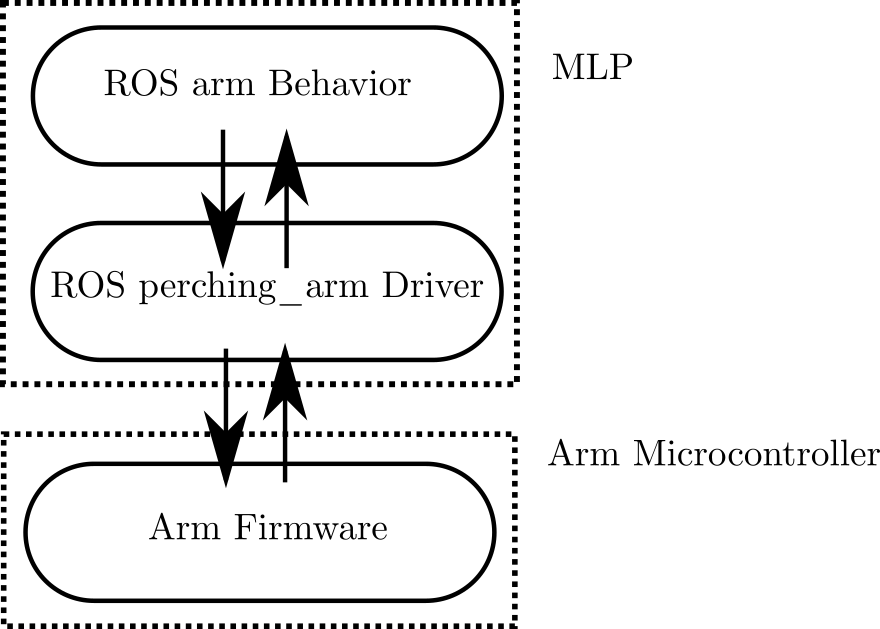
\includegraphics[width=0.8\textwidth]{img/arm_diag.png}
    \caption{The arm software flow. Note that changes to the arm interface are expected in future Astrobee code updates.}
    \label{fig:arm}
\end{figure}

\begin{markdown}
The possible actions are:

* ARM_STOP - Stop any action underway.
* ARM_DEPLOY - Deploy arm to pan = 0, tilt = 0.
* ARM_STOW - Stow arm back to its home position.
* ARM_PAN - Pan to a specific value in degrees.
* ARM_TILT - Tilt to a specific value in degrees.
* ARM_MOVE - Move to a specific pan and tilt value.
* GRIPPER_CALIBRATE - Instruct firmware to find gripper end-stops.
* GRIPPER_SET - Set the gripper to a percentage open.
* GRIPPER_OPEN - Open the gripper.
* GRIPPER_CLOSE - Close the gripper.
\end{markdown}

For actual hardware use, the arm must be started up via:

\begin{markdown}
~~~~
eps_driver_tool -power -set on $PAYLOAD
~~~~

where `$PAYLOAD` is either `pay_ba` or `pay_ta`, depending on where the arm is located.
\end{markdown}

\subsection{Firmware}
\begin{markdown}
The arm firmware is located at `submodules/avionics/src/tools/perching_arm`, but is currently NASA-only.
\end{markdown}

\subsection{Driver/Parser}
\begin{markdown}
The arm driver/command parser is located at `hardware/perching_arm`. A command-line interface for serial commanding exists:

~~~~
perching_arm_tester -o /dev/null
~~~~

This will run the serial command-line interface to the arm. For example, the following sequence can be commanded over serial:

* `m SERVO_NUM -DEG` moves SERVO_NUM to DEG degrees, [-90, 90]. Servo 0 starts at 90, Servo 1 starts at 0.
* `en g` enables the gripper
* `c 8 51 0` calibrates the gripper
* `c 8 52 0` opens the gripper
* `c 8 53 0` closes the gripper
\end{markdown}

\subsection{Command-Line Interface}
\begin{markdown}
There is also command line interface to the arm that can be used as follows:

~~~~
rosrun arm arm_tool -helpshort
~~~~

The arm's gripper must be calibrated before use. To calibrate the gripper, open it, close it and then set it to 50% open via the following sequence of commands:

    rosrun arm arm_tool -cal
    rosrun arm arm_tool -open
    rosrun arm arm_tool -close
    rosrun arm arm_tool -set 50
\end{markdown}


\subsection{Topics and Messages}

\begin{markdown}
At any point the user can inspect the internal state of the arm behavior using the following command. This command will return a sequence of numbers, which represent a time ordered sequence of states. Please refer to ```ff_msgs::ArmState``` for a mapping from numbers to states.

~~~~
rostopic echo /beh/arm/state
~~~~

If the user ever needs to manually set the arm state to a specific value, they can call the ```set_state``` service with the new state as the single argument:

~~~~
rosservice call /beh/arm/set_state 1
~~~~
\end{markdown}

\clearpage
\section{Adding New Code}

This section includes general advice on pulling new code into the Astrobee build system and running it successfully in the simulation. (The process on hardware is similar, but has additional steps including cross-compilation mentioned in Section 3. Consult the Astrobee Operations Manual for ground test instructions.) Like typical ROS development, Astrobee groups key functionality into packages but additionally tends to use nodelets (rather than nodes) to encapsulate functions within these packages. First, the process for adding a new package will be discussed.

\subsection{Adding a New Package}
\begin{markdown}
For non-NASA development, packages can be added in any directory in the `$SOURCE_DIR`, e.g., `freeflyer-shared/$MY_NEW_PACKAGE_DIR`. New directories
can be added to the existing file structure of the source code as well, but the `CMakeLists.txt` sequence must be modified to find them. 
\end{markdown}

A typical package looks like Figure \ref{fig:package}. Here the package has been named \texttt{planner\_trapezoidal} and has source code for a nodelet, a launch file to launch the package, and some supporting files for building and helping ROS to identify the package. These details are covered later in this section.

\begin{figure}[hb!]
	\centering
	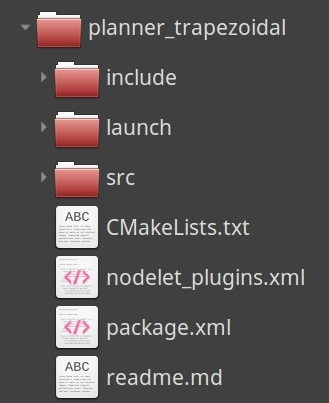
\includegraphics[width=0.5\textwidth]{img/sample_package.jpg}
	\caption{The typical package structure for an Astrobee package. Note the \texttt{nodelet\_plugins.xml}, meaning that a nodelet is used.}
	\label{fig:package}
\end{figure}
\vspace{1cm}

Note that the new package name cannot compete with the name of an existing package! If this is the case, the user must either replace the existing package's functionality entirely and turn off its compilation, or rename the new package.


\subsection{Integrating with the Build System}

\begin{markdown}
Assuming a new directory has been added, modifying the main `CMakeLists.txt`, located in `$SOURCE_DIRECTORY` would be appropriate to include the `$MY_NEW_PACKAGE_DIR` directory. Near the `if (USE_ROS)` conditional, add the desired subdirectory, e.g. `add_subdirectory($MY_NEW_PACKAGE_DIR)`. An additional `CMakeLists.txt` must be added in the newly created subdirectory and in every package in that subdirectory as well, as in Figure 12. Using e.g. `gnc` as an example, format an additional `CMakeLists.txt` in the newly added subdirectory. Place individual packages as `add_subdirectory($PACKAGE_NAME)`, and format the individual package `CMakeLists.txt`'s as usual for a ROS `CMakeLists.txt`.
\end{markdown}

\subsubsection{Custom CMakeLists.txt Commands}
In addition to the standard ROS usage of \texttt{CMakeLists.txt}, the \texttt{cmake} folder has custom CMake functions that are used in the top-level \texttt{CMakeLists.txt} and its sub-\texttt{CMakeLists.txt}'s. The important ones to note are: \texttt{CreateLibrary}, \texttt{CreateMsgTargets}, and \texttt{InstallLaunchFiles}. These custom commands are listed below, to ensure that any code written actually gets placed in the correct directories that ROS and Astrobee hardware will expect to see.


\vspace{0.5cm}
\noindent\textbf{ROS Messages}

The majority of Astrobee's message files are located in the \texttt{ff\_msgs} package, located at\\\\
\texttt{communications/ff\_msgs/msg}\\

During build, these .msg files get ROS-ified and turned into usable headers for C++. Include these in source files, e.g., \texttt{\#include <ff\_msgs/FamCommand.h>}. \\

Custom messages in a package can be installed via CMake using\\\\
\texttt{create\_msg\_targets()}


\vspace{0.5cm}
\noindent\textbf{Launch Files}

Custom launch files in a package can be installed via CMake using\\\\
\texttt{install\_launch\_files()}


\subsubsection{Comparison to Catkin}

A typical Catkin workspace and Astrobee workspace are shown in Figure \ref{fig:ws}. Catkin is normally used to produce the ROS workspace, and then to manage CMake in compiling files from \texttt{src} in \texttt{build}, and moving the products to \texttt{devel} and \texttt{install}. Astrobee's build system will place the \texttt{devel} folder inside \texttt{freeflyer-build}, and a few custom CMake scripts exist for e.g., installation of launch files. The Astrobee build process uses regular \texttt{make} called from the \texttt{freeflyer-build} folder. Rules defined in the top-level \texttt{CMakeLists.txt} in \texttt{src} make sure that some Catkin-specific functions are fulfilled.

\begin{figure}[h!]
	\centering
	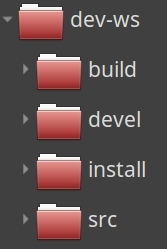
\includegraphics[width=0.3\textwidth, align=c]{img/catkin.jpg}
	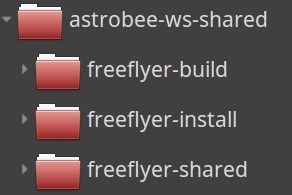
\includegraphics[width=0.5\textwidth, align=c]{img/astrobee_ws.jpg}
	\caption{A standard Catkin workspace directory (left); the typical workspace setup used by the Astrobee Flight Software (right).}
	\label{fig:ws}
\end{figure}


\subsection{Running a New Package}
\begin{markdown}
After a package gets compiled, its node(let)s and other targets are available for ROS use, as long as the ROS Astrobee workspace has been overlaid as in Section 3. A custom node executable, for example, can be launched via `rosrun $PACKAGE $NODE_EXE_NAME`. Nodelets can also be run after compilation, as specified in the nodelet subsection below.
\end{markdown}

\subsubsection{Debugging}
\begin{markdown}
- `rqt_graph` is a handy ROS tool for showing node interactions.
- `rostopic echo` can show what's being published on a certain topic.
- `rosnode $NODE info` can show what a node is interacting with.
- logging using `ROS_NODELET_DEBUG` statements is especially handy for viewing output. See the subsection below on nodelet debugging and logging.
\end{markdown}

\subsubsection{``Turning Off" a Node}
\begin{markdown}
The user can effectively turn off a node by stopping its execution from the Astrobee launch file sequence. To do so,
trace the launch file calls from `astrobee/launch` (see Section 4) and remove the desired node(let)s from execution.

To stop compilation entirely, a node(let)'s package must be removed from the chain of `CMakeLists.txt`'s.

Alternately, it is possible to just run `rosnode kill $NODE` in order to stop a node after it has been launched.
\end{markdown}



\subsection{Nodelets}

Nodelets incur no copy-passing and can therefore be more efficient than nodes. Astrobee uses them. More information on nodelets can be found \href{http://wiki.ros.org/nodelet}{here}. Nodelets have a \textit{manager} which can handle multiple nodelets and takes care of the no-copy message passing between nodelets under that manager. The user must \texttt{roslaunch} both a nodelet and its manager for code to run. (An exception: it is possible to launch standalone nodelets, mainly for debugging)

\subsubsection{Integrating a Nodelet}
The following must be included and/or modified in a package containing a nodelet in order to fully integrate it:
\begin{itemize}
	\item \texttt{nodelet\_plugins.xml} : add and fill out basic information.
	\item \texttt{package.xml} : add a nodelet dependency.
	\item \texttt{CMakeLists.txt} : create a shared library.
	\item \texttt{src} : extend the NodeHandle class and include required functions in any nodelet source code. For Astrobee, all nodelets extend from \texttt{ff\_util::FreeFlyerNodelet}.
	\item \texttt{launch file} : the main launch file (probably \texttt{MLP.launch} or \texttt{LLP.launch}) must call the nodelet and nodelet manager to start them. See \texttt{MLP.launch} for Astrobee-esque examples.
\end{itemize}

Here is an example of creating a shared library for a nodelet within \texttt{CMakeLists.txt}:

\begin{markdown}
~~~~
create_library(TARGET tumble_targ_ctl
LIBS ${catkin_LIBRARIES} ${EIGEN_LIBRARIES} common ff_nodelet
INC ${catkin_INCLUDE_DIRS} ${EIGEN3_INCLUDE_DIRS}
DEPS ff_msgs ff_hw_msgs)
~~~~
\end{markdown}

\subsubsection{Nodelet Debugging}
It is useful to run nodelets individually for debugging purposes. This can be done with a special launch file that launches the nodelet standalone, without a nodelet manager, or with a nodelet manager just like in \texttt{MLP.launch}. The user \textit{must} set their environment variables to be the same as those used in \texttt{astrobee/sim.launch}, since they will be used by \texttt{FreeFlyerNodelet}. Additionally, logging must be set appropriately as noted in the next subsection. An example standalone launch file might look like:
\begin{markdown}
	<launch>
	<arg name="robot" default="$(optenv ASTROBEE_ROBOT sim)" />
	<arg name="world" default="$(optenv ASTROBEE_WORLD iss)" />
	
	<env name="ASTROBEE_ROBOT" value="$(arg robot)" />
	<env name="ASTROBEE_WORLD" value="$(arg world)" />
	<env if="$(eval optenv('ASTROBEE_CONFIG_DIR','')=='')"
	name="ASTROBEE_CONFIG_DIR" value="$(find astrobee)/config" />
	<env if="$(eval optenv('ASTROBEE_RESOURCE_DIR','')=='')"
	name="ASTROBEE_RESOURCE_DIR" value="$(find astrobee)/resources" />
	<env if="$(eval optenv('ROSCONSOLE_CONFIG_FILE','')=='')"
	name="ROSCONSOLE_CONFIG_FILE" value="$(find astrobee)/resources/logging.config"/>
	
	<arg name="spurn" default=""/>                 <!-- Prevent a specific node   -->
	<arg name="nodes" default=""/>                 <!-- Launch specific nodes     -->
	<arg name="extra" default=""/>                 <!-- Inject an additional node -->
	<arg name="debug" default=""/>                 <!-- Debug a node set          -->
	<arg name="dds" default="false"/>              <!-- Should DDS be started     -->
	<arg name="output" default="screen"/>          <!-- Where nodes should log    -->
	
	<!-- Start a nodelet manager, if needed -->
	<node
	pkg="nodelet" type="nodelet" name="td_manager"
	args="manager"
	output="$(arg output)"/>
	
	<!-- Now inject the nodelet into the nodelet manager -->
	<node pkg="nodelet" type="nodelet" name="chaser_coordinator"
	required="false" respawn="false"
	args="load chaser_coordinator/ChaserCoordinatorNodelet td_manager"
	output="$(arg output)"/>
	
	<param name="td/instruct" type="string" value="no_action" />
	</launch>
\end{markdown}

\subsubsection{Nodelet Logging}

Nodelet logging levels must be set so that logged output is actually recorded or sent to the screen. In brief: inside a nodelet, use one of the nodelet logging macros like \texttt{NODELET\_DEBUG\_STREAM}. In \texttt{astrobee/resources/logging.config} add the specific nodelet and set the logging level to \texttt{DEBUG}:\begin{markdown}
	# TUMBLEDOCK NODELET LOGGING
	log4j.logger.ros.Astrobee./honey/chaser_coordinator    = DEBUG
	log4j.logger.ros.Astrobee./target_coordinator          = DEBUG
\end{markdown}
\vspace{0.5cm}

A bit more verbosely: usually, the \texttt{rosconsole} package is used for ROS logging. A variety of macros discussed \href{http://wiki.ros.org/roscpp/Overview/Logging}{here} are available to record information. Output can be provided to the screen using the \texttt{output = screen} argument when launching a node, or to a log file (located at \texttt{~/.ros/log}) using \texttt{output = log}. Nodelets print information using \texttt{NODELET\_DEBUG} rather than \texttt{ROS\_DEBUG} statements. Depending on the nodelet wrapper class used, the exact logging command might be different than \texttt{NODELET\_DEBUG}. For Astrobee, \texttt{NODELET\_DEBUG\_STREAM} is recommended for logging. For logging to record, the logging level for individual nodelets must be set appropriately. The global \texttt{ROSCONSOLE\_CONFIG\_FILE} is located at \texttt{astrobee/resources/logging.config}. \texttt{ff\_nodelet.launch} also has a special \texttt{debug} argument to use \\
\texttt{astrobee/resources/debug.config}, but this does not appear to be working presently. Therefore, set logging level for any nodelets in \texttt{logging.config}.

\clearpage
\section{Setting up Tests and Moving to Hardware}

After creating new autonomy functionality, integrating code into the Astrobee ecosystem, and debugging, it is time to begin thinking about setting up higher-level test coordination. There are a few major options when deciding how to run Astrobee Flight Software code:

\begin{enumerate}
    \item Use the Astrobee Android/Java API (Java/rosjava or Android APKs) to command custom nodelets/executables.
    \item Use direct ROS command-line functionality (Python or Bash scripts, or direct terminal commands).
    \item Create a custom launch file sequence (ROS launch files) to start self-managed nodelets.
    \item Integrate GDS command functionality (modification of \texttt{executive}) to capture Guest Science Commands on the MLP.
\end{enumerate}

The first method allows APKs to interface via rosjava to the general ROS ecosystem, allowing nodelets, scripts, launch files, etc. to be called as normal. Further, Astrobee Android is already integrated with GDS commanding and might be modifiable to receive custom Guest Science commands. However, this method is not very practical for simulation-only testing.

The second method is more familiar to standard ROS use, and means that simple scripts can be set up to call and execute nodelets and instructions as desired. Hardware testing integration is potentially more challenging for a true ISS experiment.

The third method relies on nodelets running passively from a standard launch sequence, e.g., by launching nodelets from \texttt{LLP.launch}. This is a good way to remain on the MLP/LLP for hardware use and run alongside the rest of the Astrobee autonomy stack, and may be combined with e.g., the second method to issue real-time commands.

Finally, the fourth method relies on integration with the GDS interface, which is one of the primary ways that Astrobee is remotely commanded. This method may be combined with Astrobee Android or MLP/LLP use, but requires capturing new commands received from GDS as well as having a working ground station executable setup. This method is also not very practical for simulation-only testing.

\subsection{Ground Data System (GDS) or Command Line?}

There is a well-defined interface for the Astrobee GDS to issue standard commands. The GDS code is open-sourced \href{https://github.com/nasa/astrobee_gds/}{here}. An open-source binary can be requested (with application) \href{https://software.nasa.gov/software/ARC-17994-1}{here}. However, the DDS communications libraries are proprietary and are not open-sourced---they are included in the requestable executable, but cannot be independently distributed or compiled from source. However, a Guest Science commanding tool mimicking actual functionality is documented \href{https://github.com/nasa/astrobee_android/blob/master/running_gs_app.md#4-guest-science-commanding}{here}. This tool can also be launched via:

\begin{markdown}
~~~~
rosrun gds_helper gds_simulator.py
~~~~
\end{markdown}

Commanding Astrobee outside of GDS and the Astrobee Android environment is somewhat more ad hoc. The steps in the following subsection provide one set of procedures for commanding Astrobee tests via rospy/roscpp on a command-line level. A few options for running tests are to incorporate high-level logic into a main test script, or to embed this logic directly in a coordinating node(s), possibly launched by a main launch file. As an example:
\begin{itemize}
    \item Main Test Script (e.g., \texttt{main.py}) : The entrypoint to running other tests, this script can perform high-level coordination with ROS. A simple Python script that starts nodes and communicates on desired topics.
    \item Main Launch File (e.g., \texttt{main.launch}) : The main launch file, launching the desired ROS nodes. A ROS launch file that starts nodes and communicates on desired topics, and may mimic the cascade of launch files shown in Section 4.
\end{itemize}


\subsection{A Sample Simulation Test}

Really, the end goal is to communicate with the desired node(let)s on the right topics at the right times. There will be multiple ways to accomplish this, but one sample procedure is provided here that has previously been demonstrated in simulation and on Astrobee ground hardware.

\begin{enumerate}
    \item Launch Astrobee, including environment setup (Main Launch File). Incorporate any custom nodes into the launch sequence. In this example, a custom node is created called \texttt{my\_ctl\_node} and is launched using a modified \texttt{sim\_info\_plan.launch}.
\begin{markdown}
~~~~
roslaunch astrobee sim_info_plan.launch dds:=false robot:=sim_pub rviz:=true
~~~~
\end{markdown}

The custom \texttt{my\_ctl\_node} must be launched. If not already configured in \texttt{sim\_info\_plan.launch}, this can be done via 

\begin{markdown}
~~~~
rosrun $DESIRED_PACKAGE $DESIRED_NODE
~~~~
\end{markdown}

\item Call scripted test number (Main Test Script). The test script should include ample time in between desired maneuvers if executing custom planning, for example.

\begin{markdown}
~~~~
rosrun test_session_tools main.py -run 0
~~~~
\end{markdown}

\item Wait for test execution. The test script will make the desired ROS calls and wait as specified---the running node(let)s will be configured as desired to interpret these test calls.
\end{enumerate}

\subsubsection{Data Recording}

Simulation data recording is as easy as using ROS' \texttt{rosbag} tool. See the rosbag \href{http://wiki.ros.org/rosbag}{documentation} for selecting the desired topics to save. Also consult the Astrobee Operations Manual.

\subsection{A Sample Hardware Test}

There are additional considerations when running a hardware test, though the basic test structure above will work and has been demonstrated in a ground test environment. See the Astrobee Operations Manual for sample ground test procedures. A future revision of this guide will include a more detailed sample hardware demonstration.

\subsubsection{Data Recording}

Hardware data recording can either be performed similar to simulation using rosbag and copied over (e.g., via \texttt{rsync}), or via NASA's Ground Data Station (GDS) GUI.
\\

\textbf{rosbag}: rosbag can be used like in simulation. This can be done through an \texttt{ssh} to Astrobee, or by setting up a proper ROS node that issues rosbag locally on the Astrobee processors via the ROS Python or C++ interface. Consult the Astrobee Operations Manual for more details.

On hardware, Astrobee also has a desired data storage directory. Consult the Astrobee Ops team for the current location of this directory, which can be automatically synced from ISS testing, for example.
\\

\textbf{GDS}: GDS can be used, which uses DDS for communications. Example profile config files are found in \texttt{\$SOURCE\_PATH/astrobee/gds\_configs/DataToDisk/}. These are placed in \texttt{\$GDS/ControlStationConfig/DataToDisk/} where the computer running GDS will display this as a recording option in the GDS GUI. These topics can then be selected for automatic download to the GDS computer from the robot.

\subsection{Notes for ISS Integration}

There are additional considerations if AFS code is eventually destined for testing on the Astrobees onboard the ISS: how will code be delivered; how can Astrobee be operated remotely; how can data be retrieved? The answers to these questions are currently being resolved as Astrobee enters some of its first on-orbit GNC test sessions in the near future.

\subsubsection{ISS Layout}

The ISS environment has a unique layout, and operations in the Japanese Experiment Module (JEM) are generally preferred. Roughly, a bounding box of $[1.5, 6.4, 1.7]\ \text{m}$ ([x, y, z], aligned with ISS coordinates), with centroid at $[10.9, -6.65, 4.9]\ \text{m}$ (also ISS coordinates) fills the internal volume of the JEM. This is not accounting for collision geometry of Astrobee, but is a rough estimate of the internal non-cluttered dimensions of the JEM, which is useful for experiment prototyping. Figure \ref{fig:iss_jem} shows these approximate dimensions.

\begin{figure}[h!]
	\begin{center}
	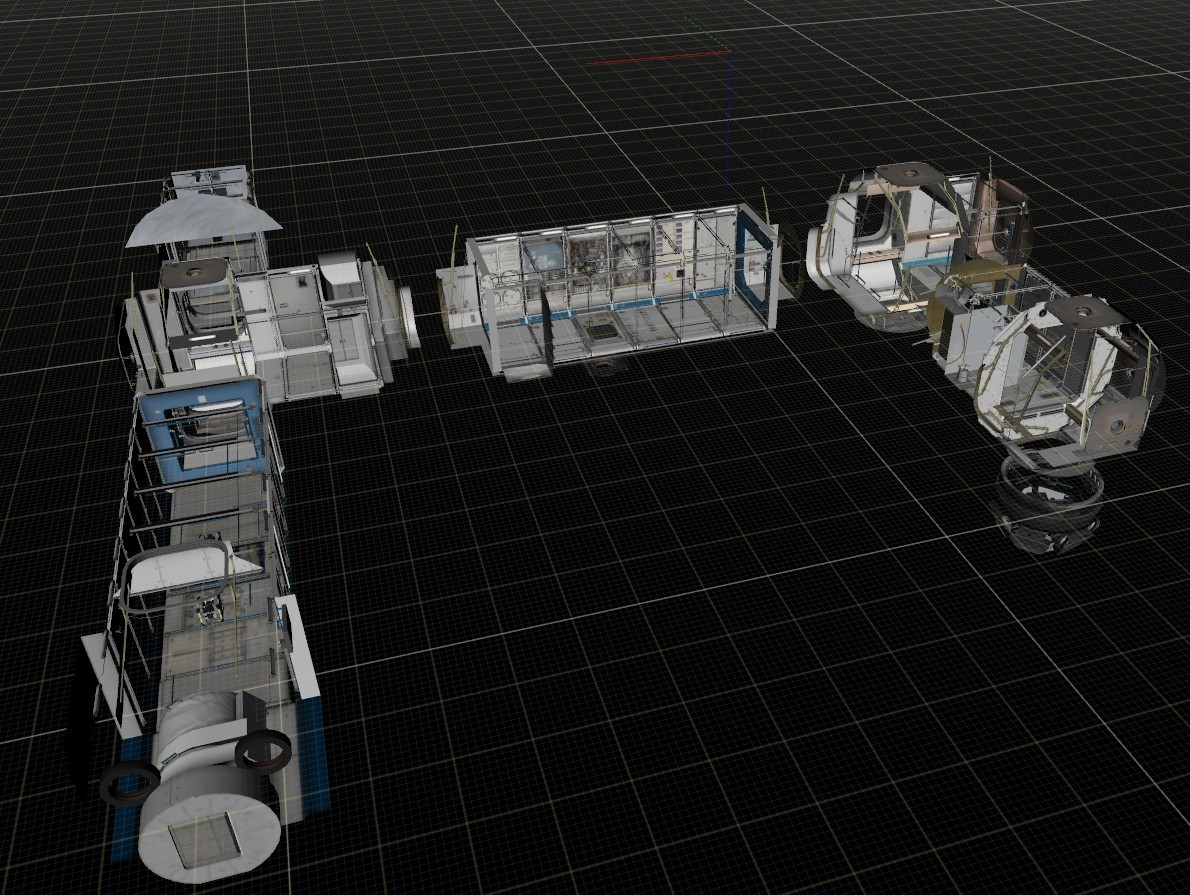
\includegraphics[width=0.8\textwidth]{img/ISS_env.jpg}\\
	\vspace{2cm}
	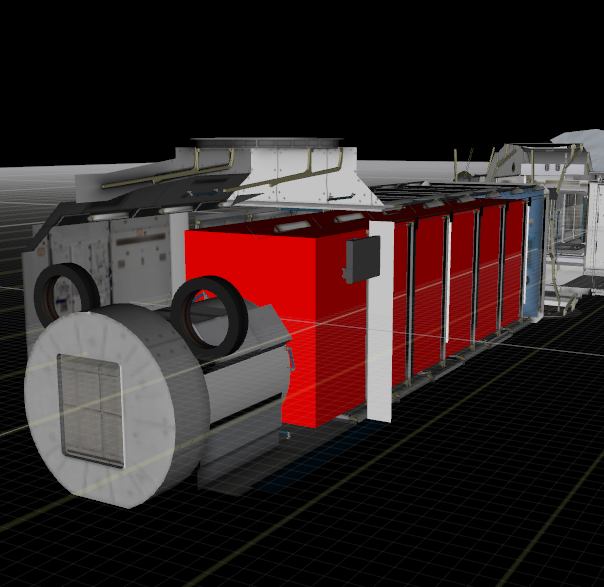
\includegraphics[width=0.8\textwidth]{img/ISS_volume.png}
	\caption{The ISS simulation environment (top), with the approximate usable volume of the JEM, in red (bottom).}
	\end{center}
	\label{fig:iss_jem}
\end{figure}

\subsubsection{Code Delivery and Upload}

Modifications to AFS intended for eventual use on ISS must be packaged as debians, the preferred method of installing and removing packages for the MLP and LLP. Section 3 has brief details on what is required to produce a debian package. In short, any external dependencies must have custom debians created, following the format used in \texttt{scripts/setup/debians}. Source code changes that have been integrated into Astrobee's build system benefit from an existing debian creation system, which uses the \texttt{debian} directory to perform packaging. Note that, as usual, cross-compilation instructions (Section 3) must be followed if the Astrobee ARM processors are the final goal for compiled code.

External library debians and a single AFS revision debian can be used to installed cross-compiled build products on the Astrobee robots. This process will also work for the Astrobee ground units; however, consult the Astrobee Ops team before making any final hardware deployment plans.

\subsection{Integration with GDS}

If using the default Astrobee Android route, GDS integration is as simple as creating custom commands for the Guest Science interface and receiving them properly from any APK code. However, if planning to run AFS code directly on the MLP/LLP it is necessary to intercept custom commands for use on the MLP/LLP. At present, this process is still being finalized; a future revision of this guide will include further detail.
\newpage
\vspace{4cm}
\begin{figure}[hb!]
	\centering
	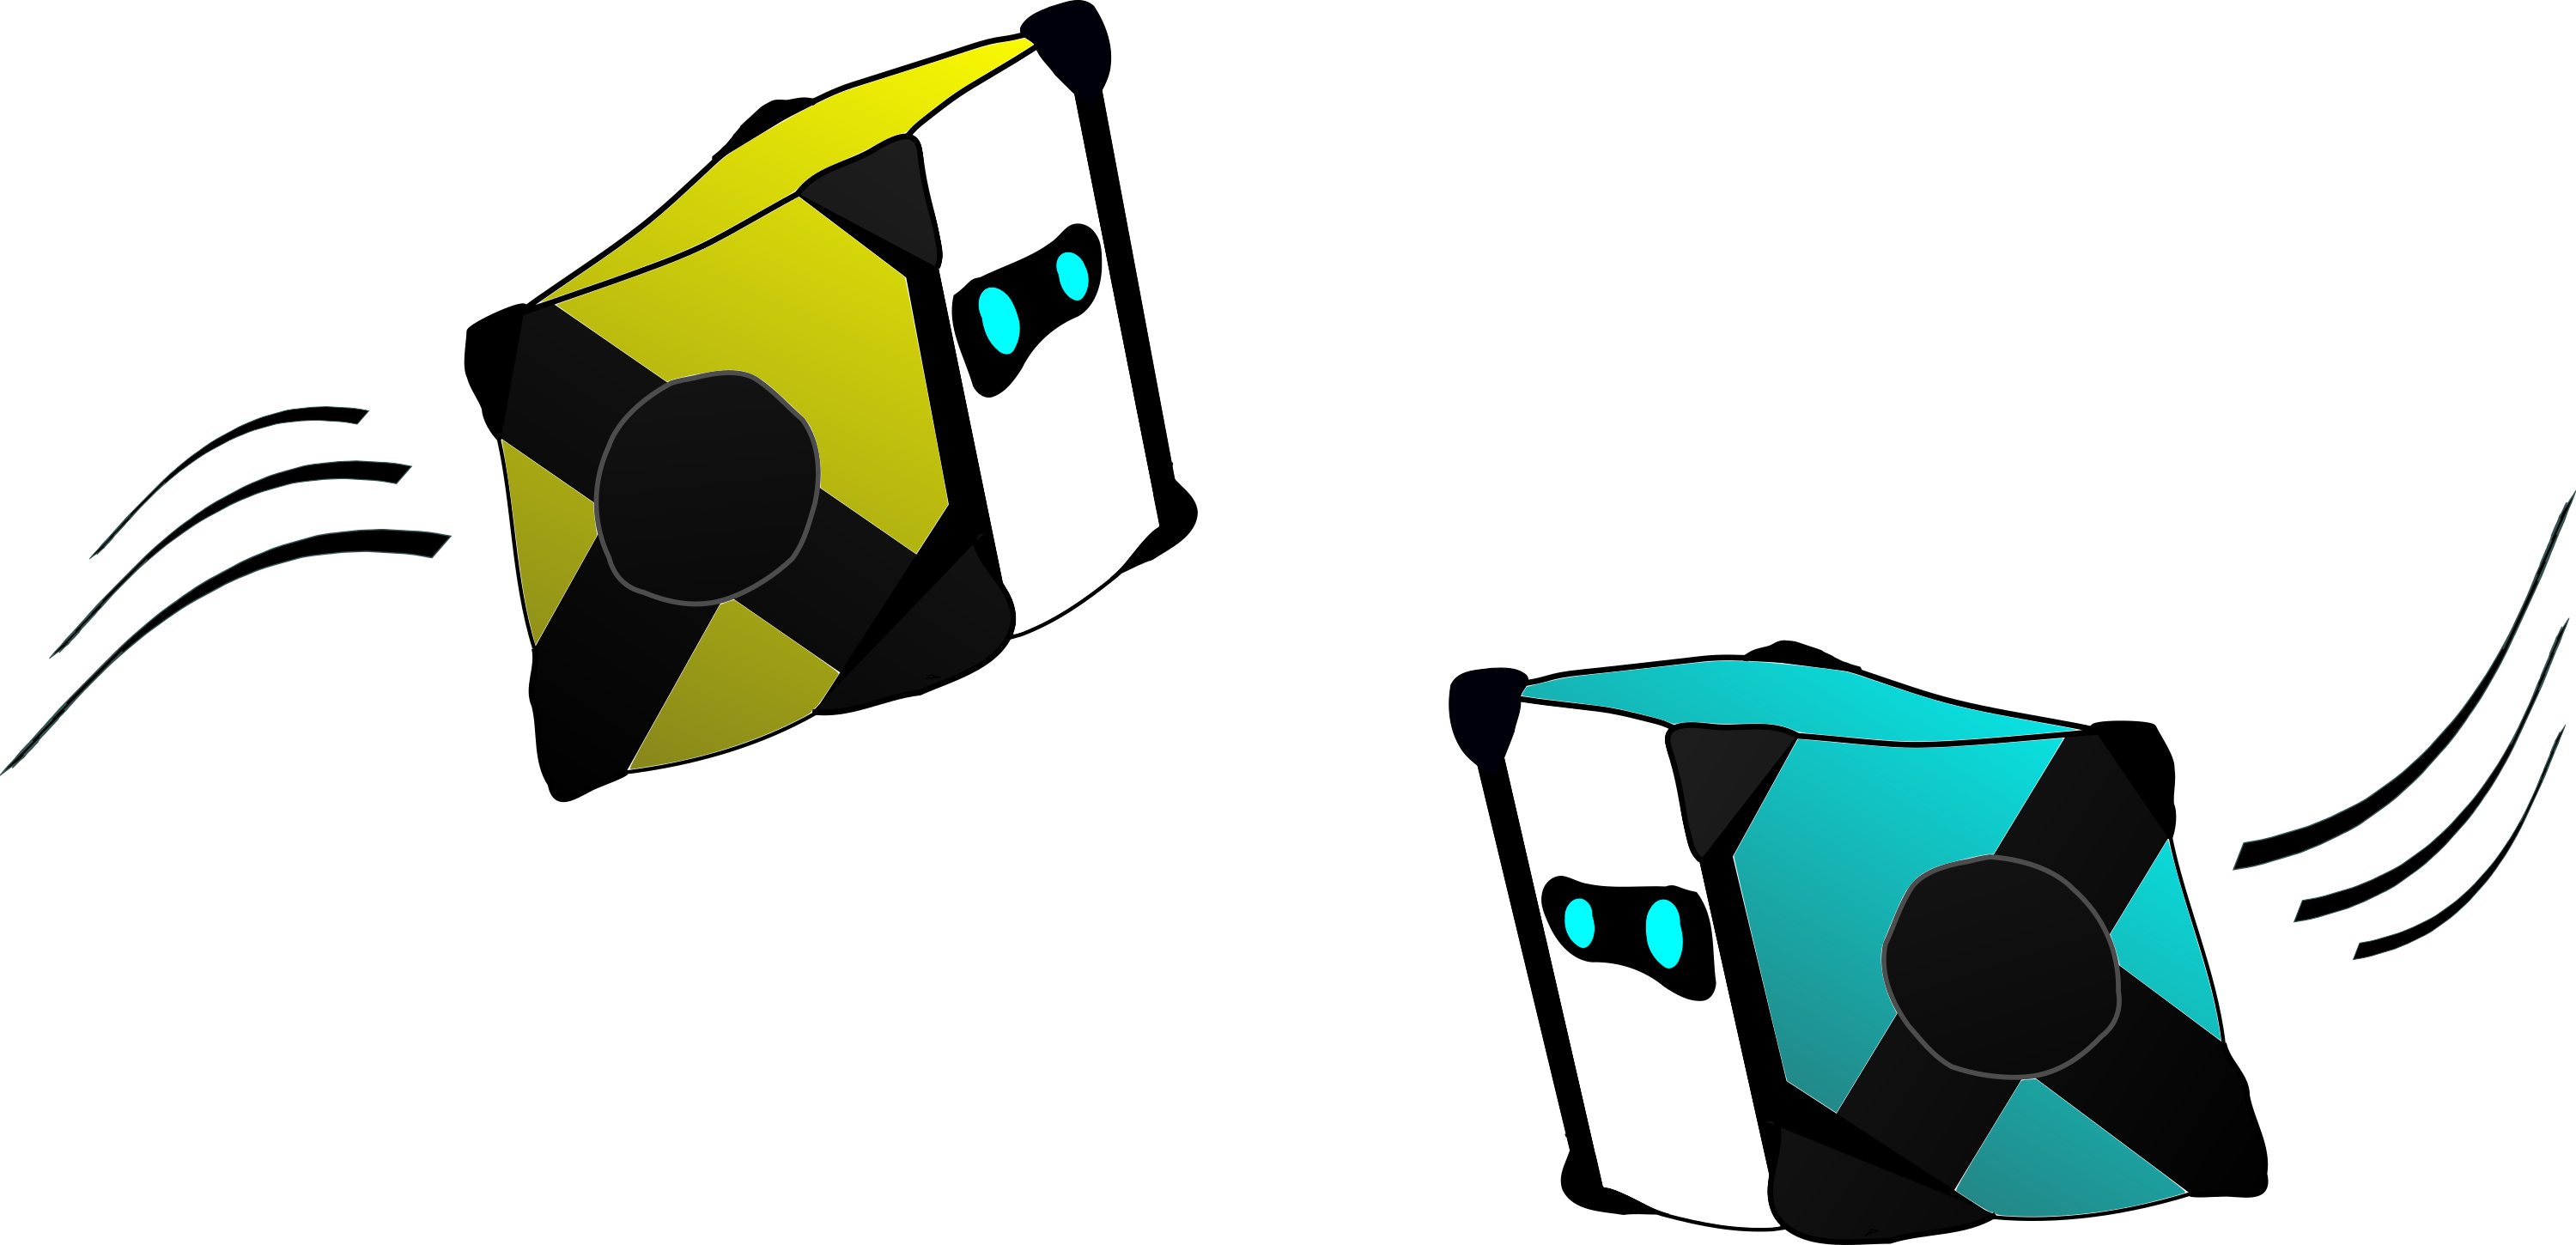
\includegraphics[width=1.0\textwidth]{img/whee.png}
\end{figure}


\clearpage
\bibliography{bib.bib}
\bibliographystyle{unsrt}
\newpage

\appendix
\section{Directory Organization}
\label{section:directory}
A cursory summary of the Astrobee Flight Software source directory is provided here for reference.\\

\begin{adjustwidth}{-1in}{-1in}
\begin{forest}
	for tree={
		font=\ttfamily,
		grow'=0,
		child anchor=west,
		parent anchor=south,
		anchor=west,
		calign=first,
		edge path={
			\noexpand\path [draw, \forestoption{edge}]
			(!u.south west) +(7.5pt,0) |- node[fill,inner sep=1.25pt] {} (.child anchor)\forestoption{edge label};
		},
		before typesetting nodes={
			if n=1
			{insert before={[,phantom]}}
			{}
		},
		fit=band,
		before computing xy={l=15pt},
	}
[freeflyer
	[astrobee: "primary entry point" into the AFS: many launch files; config files; etc.
		[config: configuration files]
		[launch: main launch file cascade for AFS]
		[plans: holds plans which are built using the Ground Data System (GDS) user interface tool]
		[resources: all non-LUA resources used by nodes in the system (e.g. logging)]
		[scripts: bash script to print out the environment variables; launch GDS]
	]
	[cmake: custom cmake functions for Astrobee build system]
	[communications: DDS and ROS message definitions]
	[debian: files for setting up a debian of the AFS]
	[description: files describing inertial properties and environments for simulation
		[description: ROS URDFs used to describe Astrobee in simulation]
		[media: robot geometry; skins; etc.]
	]
	[doc: tools for AFS documenation]
	[external: gtest debugging tools]
	[gnc: GNC nodelets; mainly autocoded
		[ekf: extended Kalman filter uses IMU and CV measurements from localization subsystem]
		[ctl: calculates forces and torques to meet requirements of mobility subsystem]
		[fam: force allocation module (a mixer to provide vent open angles)]
		[sim\_wrapper: a wrapper for using the GNC subsystem in simulation]
		[gnc\_autocode: thin C++ wrapper around the auto-generated C functions]
		[matlab: the original GNC Matlab/Simulink code]
	]
	[hardware: drivers etc. for hardware control]
]
\end{forest}
\end{adjustwidth}

\clearpage
\begin{adjustwidth}{-1in}{-1in}
\begin{forest}
	for tree={
		font=\ttfamily,
		grow'=0,
		child anchor=west,
		parent anchor=south,
		anchor=west,
		calign=first,
		edge path={
			\noexpand\path [draw, \forestoption{edge}]
			(!u.south west) +(7.5pt,0) |- node[fill,inner sep=1.25pt] {} (.child anchor)\forestoption{edge label};
		},
		before typesetting nodes={
			if n=1
			{insert before={[,phantom]}}
			{}
		},
		fit=band,
		before computing xy={l=15pt},
	}
[freeflyer
	[localization: feature detection algorithms which are then integrated into the EKF]
	[management: system monitoring and executive tools; FSMs]
	[mobility: tools that enable waypoint following within constraints
		[choreographer: manage motion requests from client nodes and manage mobility]
		[mapper: maintains a representation of the environment]
		[mobility: mobility tools like teleop]
		[planner\_qp: quartic polynomial planner]
		[planner\_trapezoidal: "straight line" trapezoidal planner]
	]
	[scripts: scripts for running AFS on hardware; setting up; etc.]
	[shared: functions used between different packages; headers; etc.]
	[simulation: all code related to the simulation/Gazebo; plugins; worlds; etc.]
	[submodules: significantly large codebases used by Astrobee: NASA internal]
	[tools: debugging tools; visualizers; helpers]
	[wdock]
]
\end{forest}
\end{adjustwidth}

\clearpage
\section{Sample Non-NASA Hardware Setup, Building, and Running the Flight Software}
\label{app:charles}

This section describes the specific code and instructions used to operate the MIT Space Systems Laboratory's ground Astrobee. The SSL Astrobee is currently being built to provide preliminary ground tests for later experiments using NASA's ISS Astrobees. It is generally similar to NASA's Astrobees, but there are a few notable differences. Details on the SSL robot processors are shared below, and the unique steps to build and run the code on the SSL robot are also included---the process of adapting the Astrobee Flight Software might prove useful to other hardware builds.

\subsection{Processors}
Like the NASA Astrobees, the SSL Astrobee includes two processors for running the main Astrobee code. The LLP is the exact same processor type as NASA's, while the MLP is a newer version of NASA's (the original NASA MLP is no longer manufactured). 

\subsubsection{Mid-Level Processor}
The SSL robot runs Astrobee MLP code on the Snapdragon 820 (APQ8096) based Inforce 6601 Micro System on Module\footnote{https://www.inforcecomputing.com/products/system-on-modules-som/qualcomm-snapdragon-820-inforce-6601-micro-som}. The MLP is an ARM64 computing platform with four cores in dual clusters: two cores operate at 2.2GHz and the other two operate at 1.6GHz. It has 4GB of RAM and 64GB of disk space. The development board includes USB, Ethernet, and HDMI connections, as well as WiFi capabilities. The MLP is kept on the development board for easy setup and debugging. Then, the MLP is transferred to the MLP/HLP carrier board on the Astrobee as part of the core module PCB stack.

The Inforce 6601 runs either an Android or Linux Debian OS. Since Astrobee needs to run in a Linux environment with ROS, the SSL robot's MLP is running the Debian 10.5 (``buster'') operating system. A specific Inforce 6601 broad support package was downloaded from the Inforce TechWeb site\footnote{https://inforcecomputing.com/techweb/} (version 1.1). So far, this operating system has been compatible with Astrobee software and uses the ROS ``noetic'' distribution. The TechWeb has resources for installing the operating system and troubleshooting basic issues. Most commands can be run by connecting the board to a monitor via HDMI and using its minimal desktop environment. The WiFi typically works out of the box. Small issues can come up and can often be solved by the following commands:
\begin{markdown}
~~~~
sudo nano /etc/NetworkManager/NetworkManager.conf
~~~~
\end{markdown}
Change the line ``managed=false'' to ``managed=true''. Then run:
\begin{markdown}
~~~~
sudo service network-manager restart
~~~~
\end{markdown}


\subsubsection{Low-Level Processor}
The SSL robot runs Astrobee LLP code on the Wandboard Dual IMX6 processor\footnote{https://www.wandboard.org/products/wandboard/WB-IMX6U-BW/}. The LLP is an ARM Cortex-A9 platform with two cores, both running at 1GHz. It has 1GB of RAM and, via a microSD card, 64GB of disk space. Like the MLP, the development board has USB, Ethernet, and HDMI connections. However, it does not have WiFi capabilities. The LLP is eventually transferred to the LLP carrier board as part of the Astrobee core module PCB stack. Note that the processing and memory capabilities of LLP are significantly less than the MLP.

It is straightforward for the Wandboard to run Ubuntu 16.04, which is the most suitable OS for Astrobee software. The board OS image and setup steps can be found on the Wandboard website\footnote{https://www.wandboard.org/downloads/}. As such, the LLP runs the ROS ``kinetic'' distribution. Like the MLP, most commands can be run using an HDMI connection, monitor, and a minimal desktop environment. It is typically useful to have an Ethernet connection by sharing a host PC's network connection\footnote{https://askubuntu.com/questions/169473/sharing-connection-to-other-pcs-via-wired-ethernet}.

\subsection{Setup and Building Code}
This section outlines the steps to download, build, and install Astrobee code on the actual MLP and LLP hardware. Note that modifications are made for the specific processors and operating systems used at the MIT SSL, and differ somewhat from stock Astrobee.

\subsubsection{SSL Source Code}
An SSL-specific version of Astrobee software can be found within the SSL GitHub repository\footnote{https://github.mit.edu/SSL/Astrobee/tree/hardware}. This source code is mostly the same as NASA's. The differences generally concern the accomodation of the MLP Debian OS and its ROS ``noetic'' distribution, specific IP address/network configurations, a library to run the VN-100 IMU (which is different than NASA's IMU), and localization maps for the SSL. 

\subsubsection{MLP Build and Installation}
Here are the steps to building and installing updated source code on the MLP (all commands via a terminal on the MLP):
\begin{enumerate}
    \item Pull the SSL/hardware repository using the MLP's WiFi capabilities.
    \item Set the source, build, and install paths as necessary.
    \item Configure the build using the following command, run from the source directory:
    \begin{markdown}
    ./scripts/configure.sh -l -F -D -R -s -b $BUILD_PATH -p $INSTALL_PATH
    \end{markdown}
        The ``-s'' option sets the configuration specifically to build on the MLP. The ``-F'', ``-D'', and ``-R'' options disable the PicoFlexx driver, DDS driver, and QP planner, respectively, which are currently not supported for hardware.
    \item Change directories via the build path, and build the code using the following command:
    \begin{markdown}
    make -j4
    \end{markdown}
    The ``j4'' option ensures a fast build without over-stressing the memory and performance capabilities of the MLP.
    \item Install the built code:
    \begin{markdown}
    make install
    \end{markdown}
    \item Set the freeflyer target variable to ``mlp'' in line 80 of  \texttt{scripts/install\_to\_astrobee.sh}
    \item Transfer the installed files to the \texttt{/opt} folder, which is where Astrobee expects to find the binaries. From the source folder:
    \begin{markdown}
    ./scripts/install_to_astrobee.sh $INSTALL_PATH$ ssl
    \end{markdown}
\end{enumerate}

Note that the MLP IP address may need to be updated depending on the WiFi configuration. This can be set in scripts/deploy/constants.sh (make sure to coordinate the IP address with the ``ssl'' robot). To test this connection, make sure the MLP can ping its own WiFi address.

\subsubsection{LLP Build and Installation}
The LLP's processing capabilities are significantly less powerful than the MLP. As such, a large portion of the Astrobee software cannot be built natively on the processor (it will run out of memory when trying to compile big localization or mobility source files). Normally, this issue is resolved by cross-compiling on a PC for the LLP's ARM architecture. However, the cross-compilation toolchain and rootfs are accessible only for NASA users. 

The SSL resolves this issue by copying the source directory to the LLP via \texttt{rsync}. Then, a specific LLP configuration option is set to prevent compilation of Astrobee subsystems that do not run on the LLP. Fortunately, the LLP-specific code components of Astrobee software (namely the hardware drivers and GNC loop) can be built natively on the LLP. Here are the steps for building and installing Astrobee software on the LLP:
\begin{enumerate}
    \item From the source folder on a PC, copy the \texttt{SSL/hardware} freeflyer directory to the LLP, excluding the \texttt{debians} folder:
    \begin{markdown}
    rsync -rlug --exclude '/path/to/source/freeflyer/scripts/setup/debians' 
    /path/to/source/freeflyer astrobee@{LLP_IP_ADDRESS}:/home/astrobee/ssl_ws
    \end{markdown}
    \item Set the source, build, and install paths as necessary. This step and all future steps are run on an LLP terminal.
    \item Configure the build using the following command, run from the source directory:
    \begin{markdown}
    ./scripts/configure.sh -l -F -D -R -w -b $BUILD_PATH -p $INSTALL_PATH
    \end{markdown}
    The ``-w'' option sets the configuration specifically to build on the LLP.
    \item Change directories via the build path, and build the code using the following command:
    \begin{markdown}
    make -j1
    \end{markdown}
    The ``j1'' option ensures the LLP will not run out of memory. This results in a fairly slow build, but this is offset by the fact that the LLP only builds a portion of the code.
    \item Install the built code:
    \begin{markdown}
    make install
    \end{markdown}
    \item Set the freeflyer target variable to ``llp'' in line 79 of  \texttt{scripts/install\_to\_astrobee.sh}
    \item Transfer the installed files to the \texttt{/opt} folder, which is where Astrobee expects to find the binaries. From the source folder:
    \begin{markdown}
    ./scripts/install_to_astrobee.sh $INSTALL_PATH$ ssl
    \end{markdown}
\end{enumerate}

Currently, the LLP IP address is set and remains constant, as it only is used for computer-computer Ethernet connections. However, it can be updated in the same manner as the MLP IP address if necessary.

\subsection{Running Code on the Robot}
Now that the code is built and installed to the \texttt{/opt} folder of both the MLP and LLP, the Astrobee code can be run with a host PC as the ROS master. This section will walk through an example launch process to run the IMU.

\subsubsection{Network}
To begin, connections must be established with both the MLP and LLP in the ROS framework. SSH keys of remote machines must reside in ``known\_hosts'' to enable their use in the ROS framework. First, double-check that, from a host PC, you can ssh into both the LLP and MLP using 
\begin{markdown}
~~~~
ssh linaro@{MLP_IP_ADDRESS}  
ssh astrobee@{LLP_IP_ADDRESS}
~~~~
\end{markdown}

Then, \texttt{ssh} into each processor and force it to use the RSA key algorithm, which is required by ROS. Doing this with both machines will enable their SSH keys to be used by ROS:
\begin{markdown}
~~~~
ssh linaro@{MLP_IP_ADDRESS} -oHostKeyAlgorithms='ssh-rsa' 
ssh astrobee@{LLP_IP_ADDRESS} -oHostKeyAlgorithms='ssh-rsa' 
~~~~
\end{markdown}

At this point, both machines should be networked and enabled for ROS. Other ROS networking issues can be resolved through the ROS documentation\footnote{http://wiki.ros.org/ROS/NetworkSetup}. If issues persist, check the \texttt{ROS\_MASTER\_URI} variable and make sure it matches across the PC, MLP, and LLP. The proper \texttt{ROS\_MASTER\_URI} can be set in the host \texttt{.bashrc} script.


\subsubsection{Launching}
Having set up the connection, it is relatively simple to launch the Astrobee Flight Software using the MLP and LLP. From the host PC, execute the following command after setting the ROS environment:
\begin{markdown}
~~~~
roslaunch astrobee astrobee.launch llp:={LLP_IP_ADDRESS} mlp:={MLP_IP_ADDRESS}  
nodes:=vn100_imu
~~~~
\end{markdown}
The inclusion of \texttt{vn100\_imu} as an extra node argument will automatically launch the IMU if it is connected to the LLP. Upon launching the software, all of the nodelet managers will launch on the actual LLP and MLP IP address from the host PC terminal. In a separate terminal on the host PC, the following command can be run to view the IMU's output:
\begin{markdown}
~~~~
rostopic echo /hw/imu
~~~~
\end{markdown}

To launch all nodes on a completed robot, the following command can be run:
\begin{markdown}
~~~~
roslaunch astrobee astrobee.launch drivers:=true robot:=honey llp:={LLP_IP_ADDRESS}
~~~~
\end{markdown}
Note that only the LLP IP address needs to be specified in this case. This is because on a completed robot, there is an internal network between the LLP and MLP. The LLP serves as the ROS master in this case. This case also launches all hardware drivers.

The simulator can also be launched with the processor network. This essentially creates a hardware-in-the-loop simulation, where all nodes are running on the respective machines but the ``robot" is still in the simulation environment. This can be done by
\begin{markdown}
~~~~
roslaunch astrobee sim.launch llp:={LLP_IP_ADDRESS} mlp:={MLP_IP_ADDRESS}
~~~~
\end{markdown}

For more information on different ways to launch Astrobee software, see the \texttt{astrobee} documentation page on the NASA GitHub\footnote{https://github.com/nasa/astrobee/tree/master/astrobee}.

\subsubsection{VN-100 IMU}

The SSL robot uses a VectorNav-100 IMU\footnote{https://www.vectornav.com/products/vn-100} instead of NASA's normal Epson IMU. This is because NASA's Epson IMU is hard to acquire and also very expensive. As such, the SSL source code repository has the necessary modifications to run the VN-100 IMU on Astrobee. Fortunately, the VN-100 IMU has a straightforward library online that can be built as a part of Astrobee's software (see the SSL repository). The modified IMU nodelet simply accepts incoming data from the IMU and publishes the necessary data that Astrobee's EKF requires.

The latency in the USB connection between the VN-100 IMU and the processor must be reduced in order to meet Astrobee's EKF requirements. This can be done by running the \texttt{usb\_help.sh} script from the SSL source repository on the processor.


\clearpage
\section{ROS Tips}

These are some useful ROS tips that will be updated from time-to-time in future guide revisions.

\begin{itemize}
    \item Adding and removing ROS packages is often made very simple since packages are commonly packaged as debians and made available via apt. The typical naming convention is \begin{markdown}
	sudo apt-get install ros-DISTRIBUTION-PACKAGE_NAME
	
	sudo apt-get install ros-kinetic-rqt-logger-level
\end{markdown}

Make sure to run a \texttt{rosdep install} to get any missing packages that the new package depends on.

\item Occasionally, rostime will \textit{not} work at all after a shutdown of the Astrobee sim. This is a hard error to catch, and can be solved by restarting \texttt{roscore}.
\end{itemize}

\end{document}
